\section{Kết quả và kết luận}

Tiến hành thực nghiệm thuật toán K-Means với các giá trị \(k\) khác nhau để giảm số màu của ảnh, đồng thời phân tích chất lượng kết quả nén dựa trên các yếu tố như chất lượng ảnh trực quan, thời gian thực thi và số vòng lặp hội tụ.

\subsection{Chất lượng hình ảnh nén theo số màu}

Kết quả ảnh nén với số lượng màu \(k=3, 5, 7, 9\) được thể hiện dưới đây, đồng thời so sánh trực quan giữa hai phương pháp khởi tạo centroid: \textit{random} và \textit{in\_pixels}.

\begin{figure}[H]
  \centering
  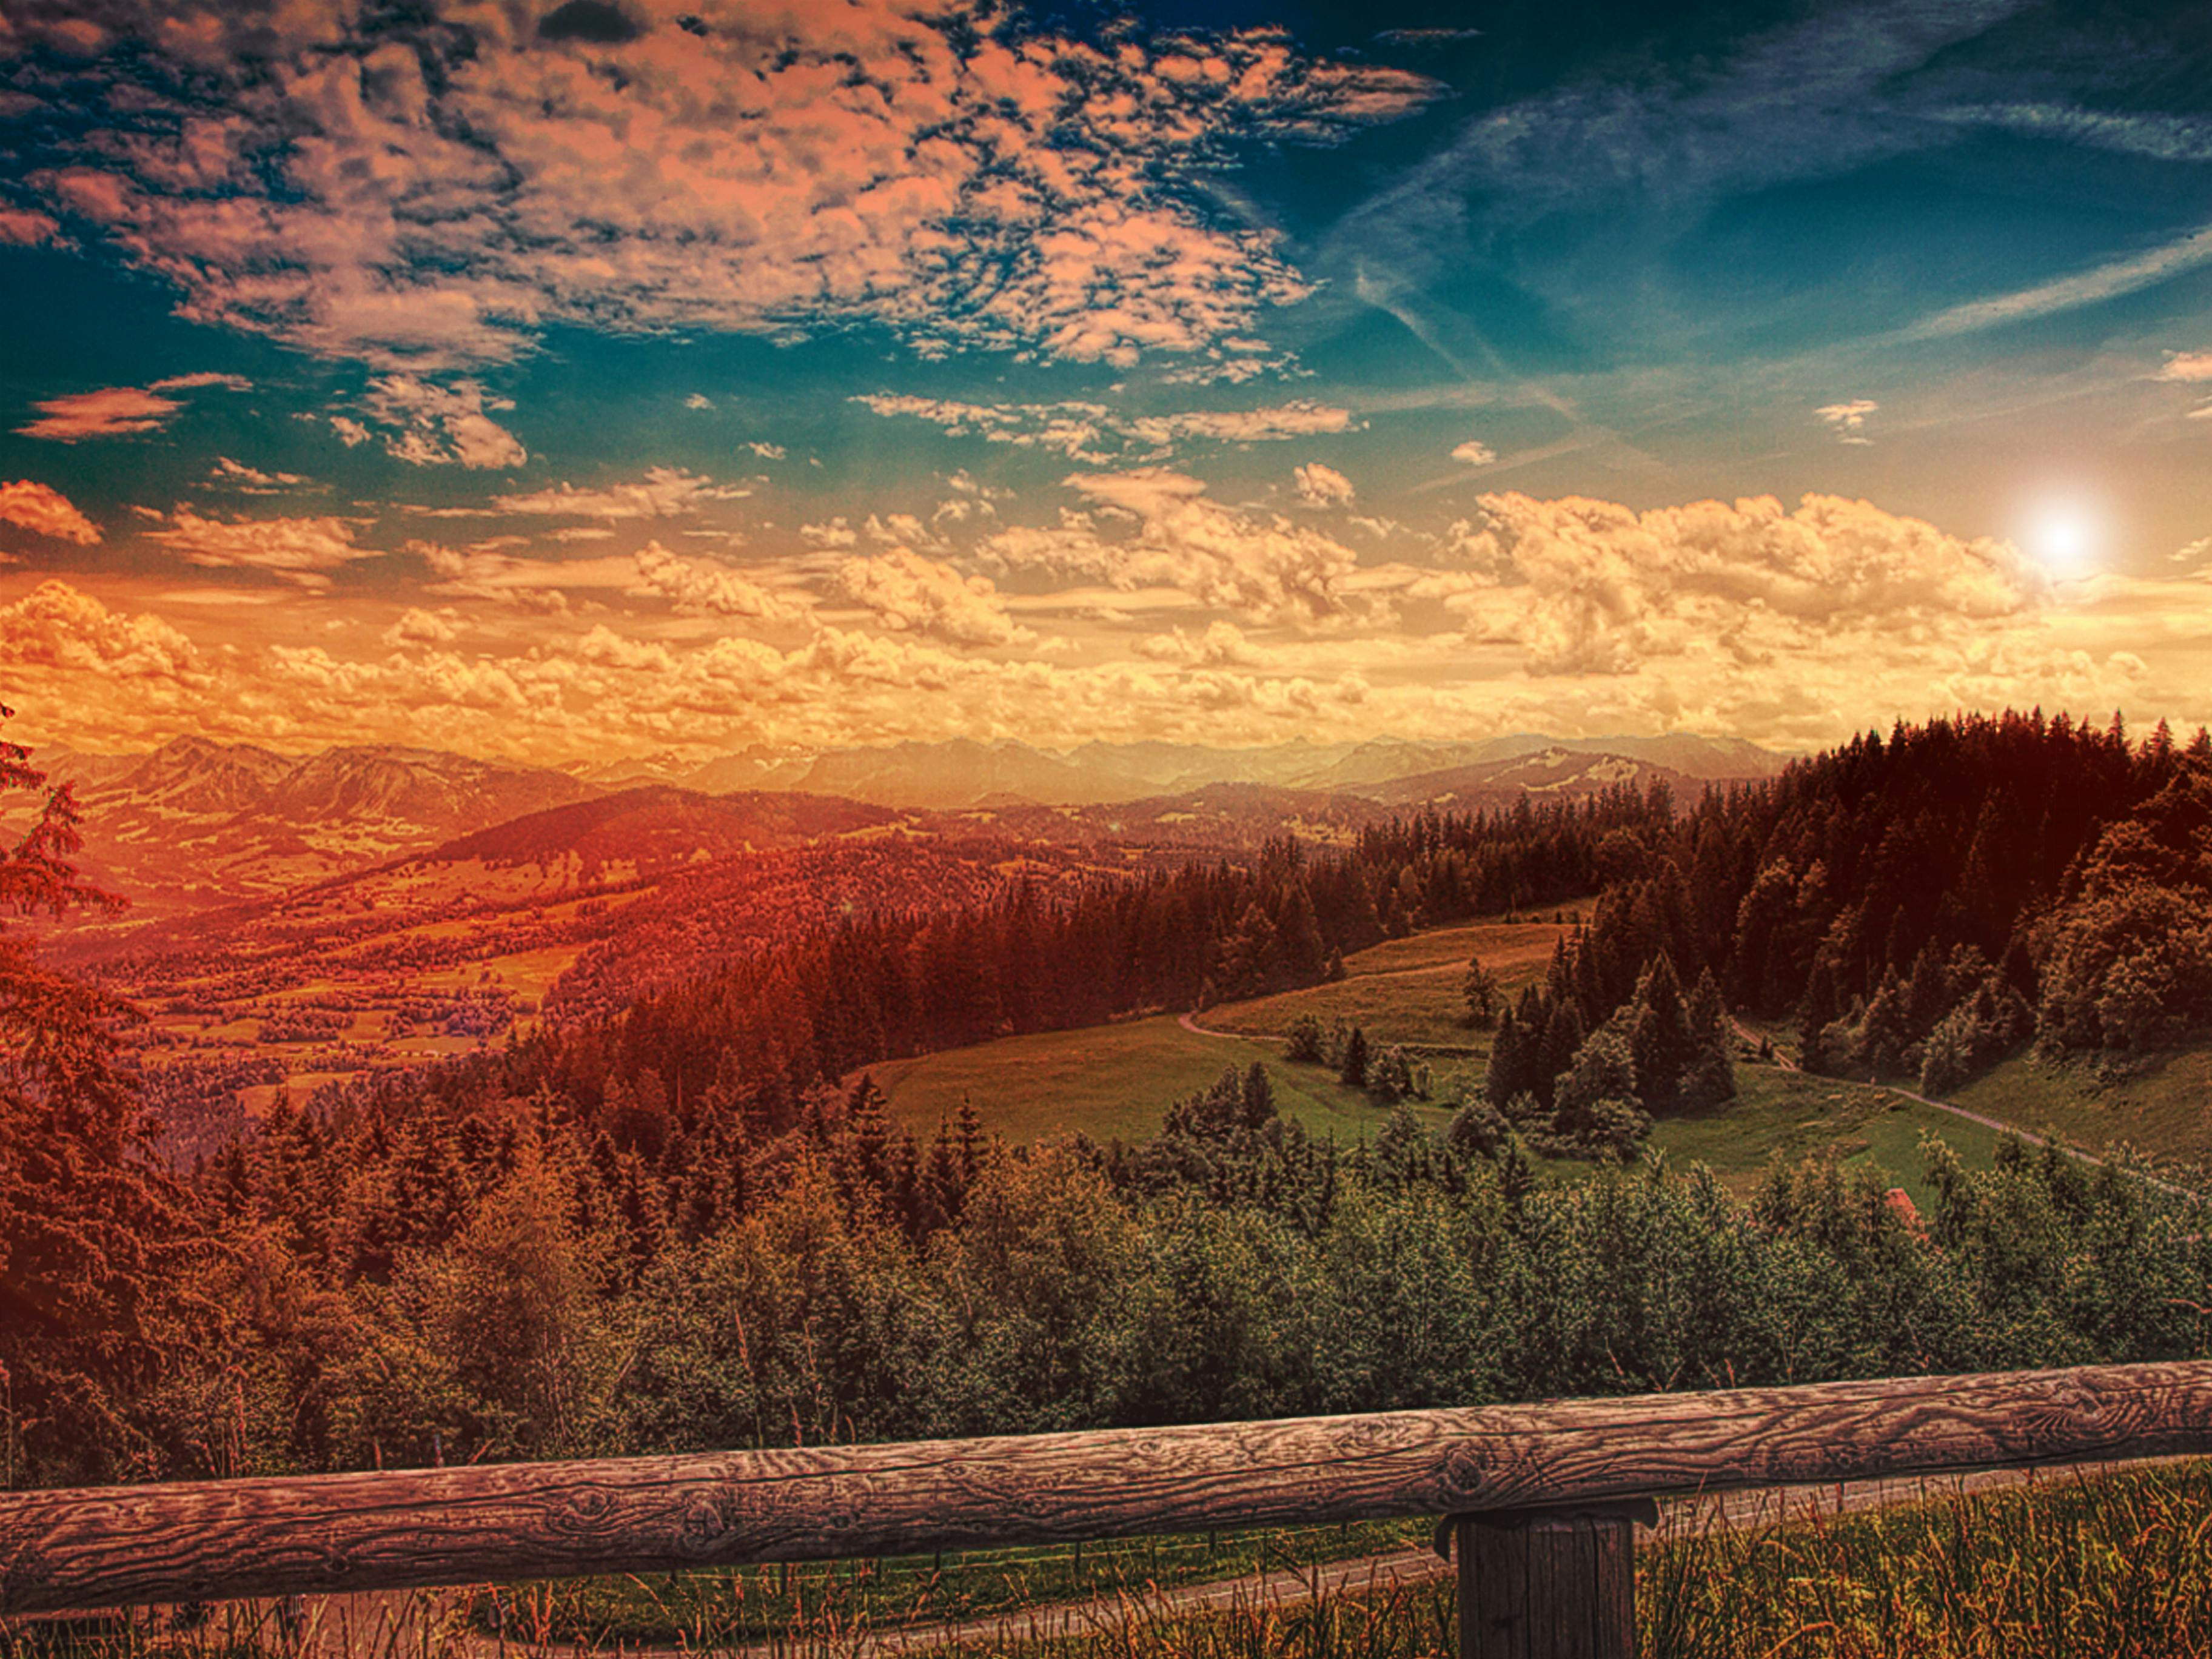
\includegraphics[width=0.6\textwidth]{imgs/original.jpg}
  \caption{Ảnh gốc dùng để so sánh nén màu.}
  \label{fig:original}
\end{figure}

\begin{figure}[H]
  \centering
  \subfloat[random]{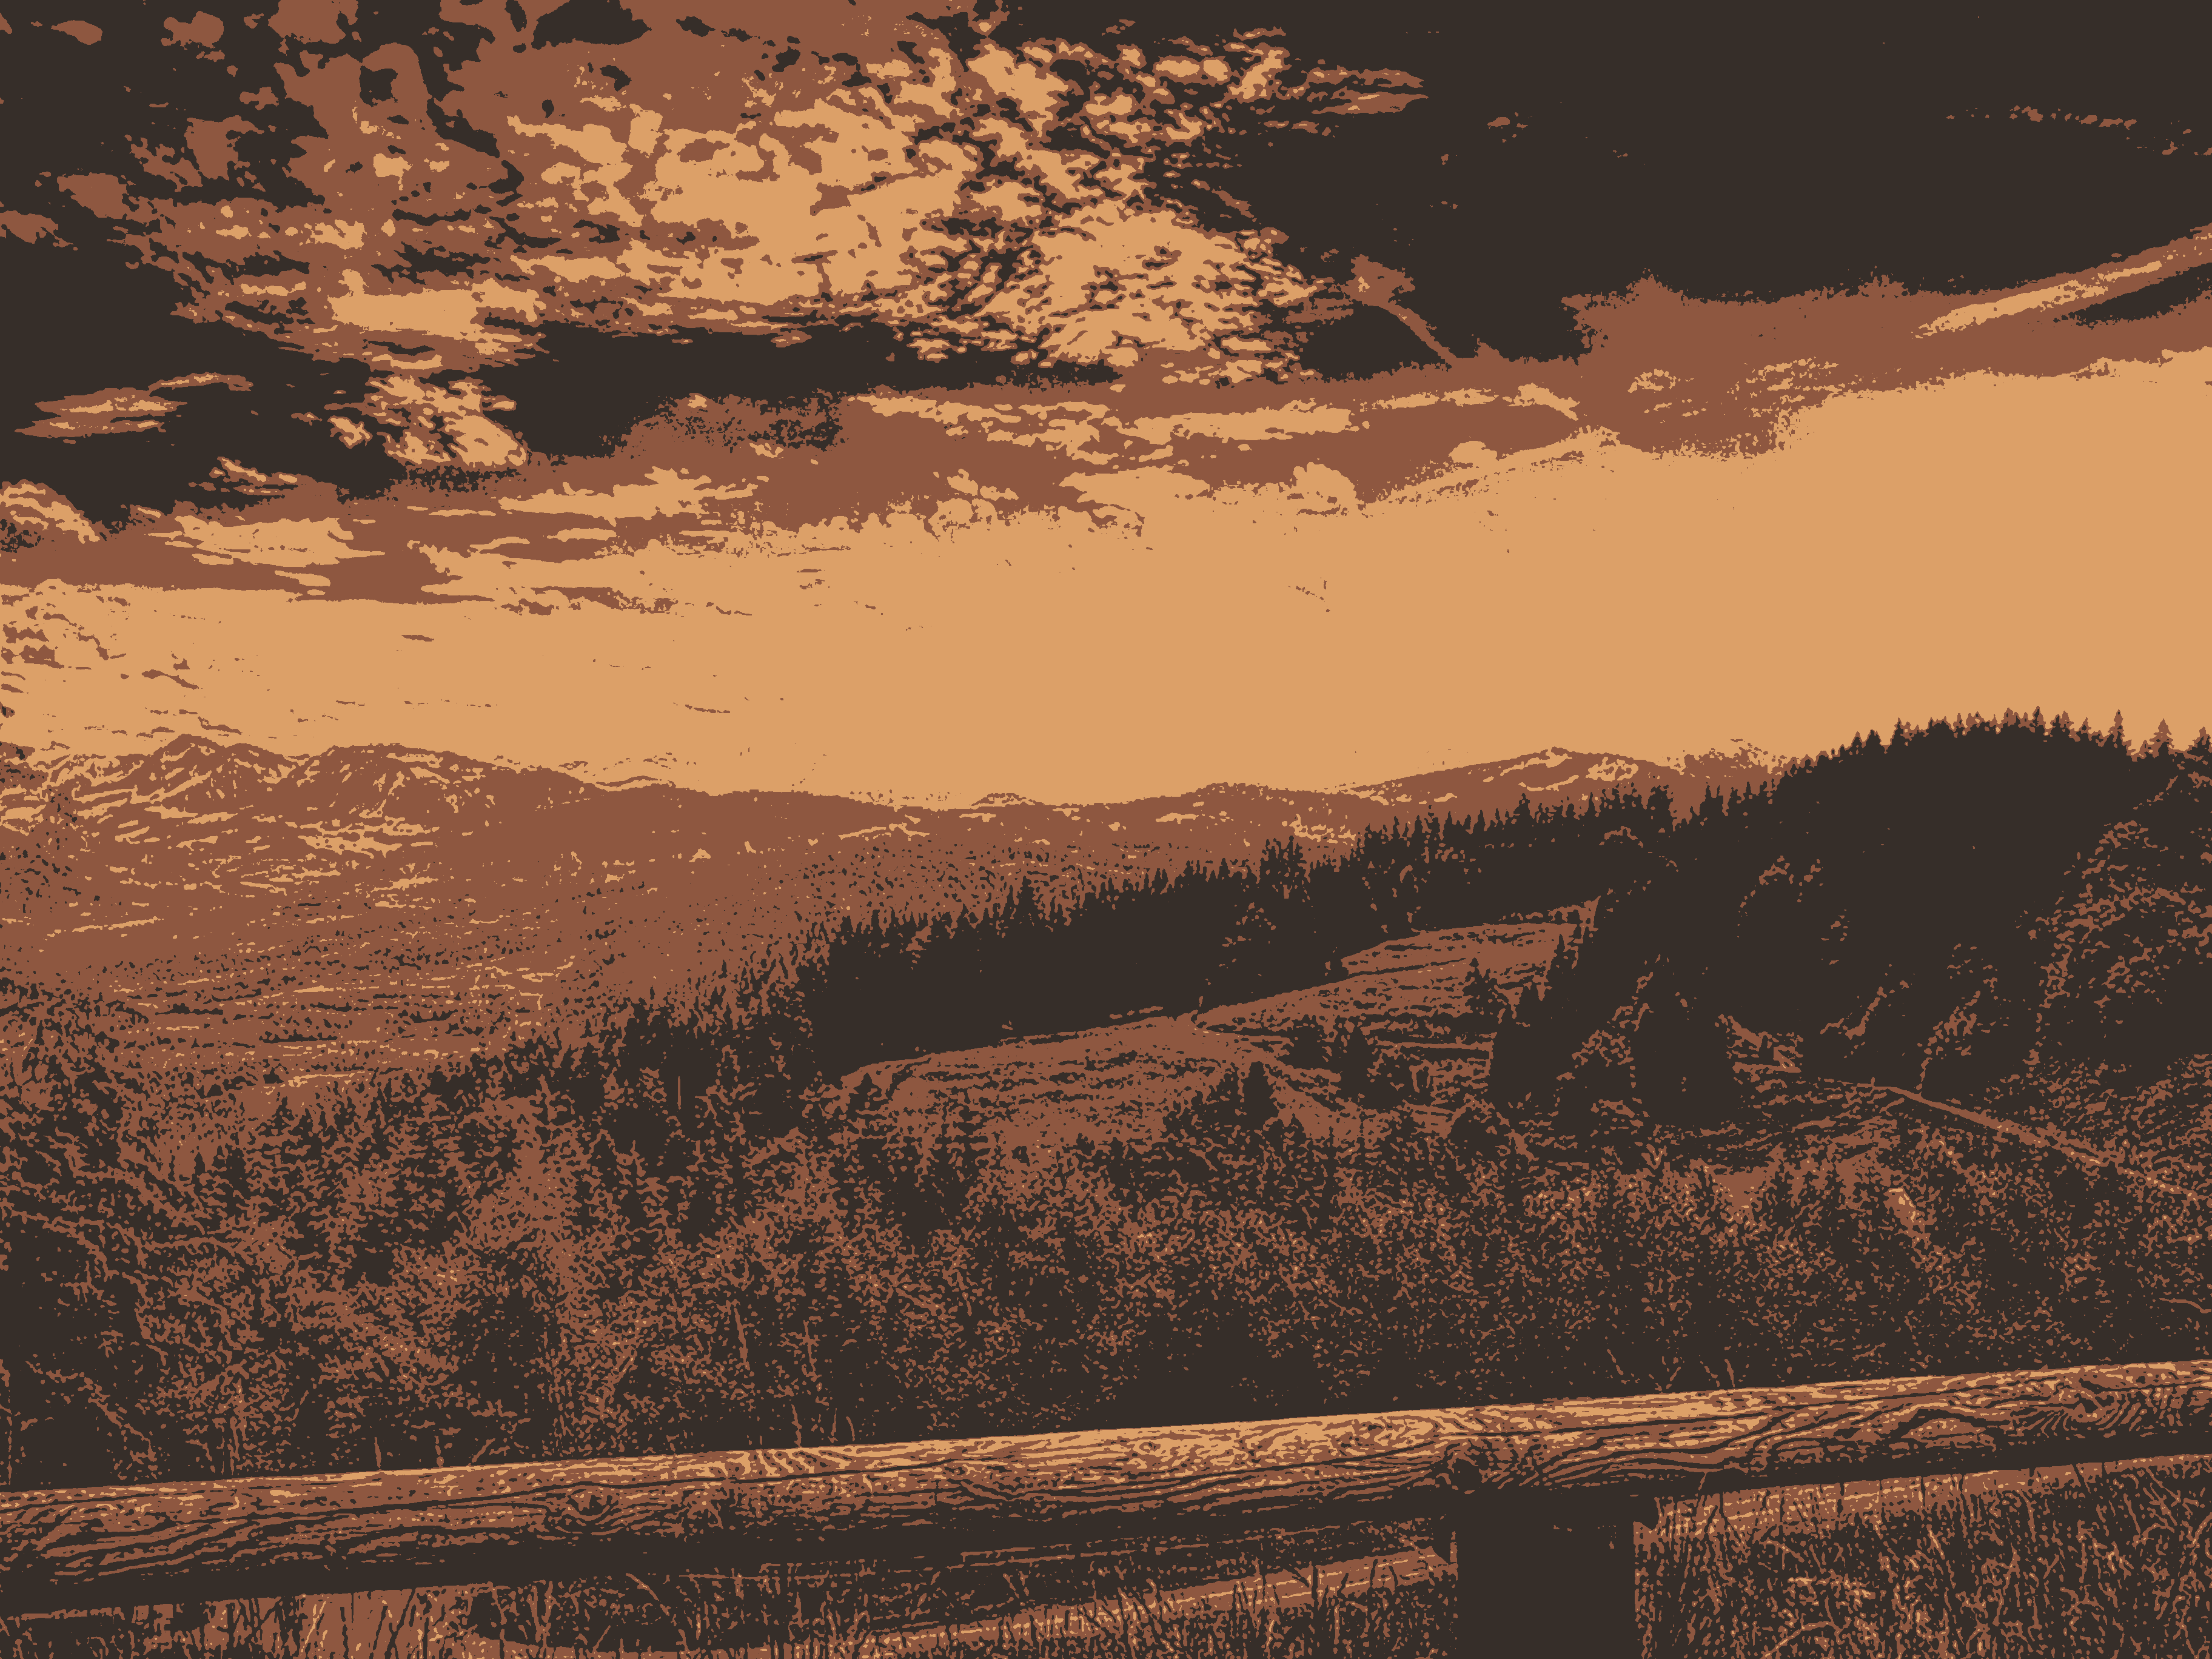
\includegraphics[width=0.45\textwidth]{imgs/output/k3_random.png}}
  \hfill
  \subfloat[in\_pixels]{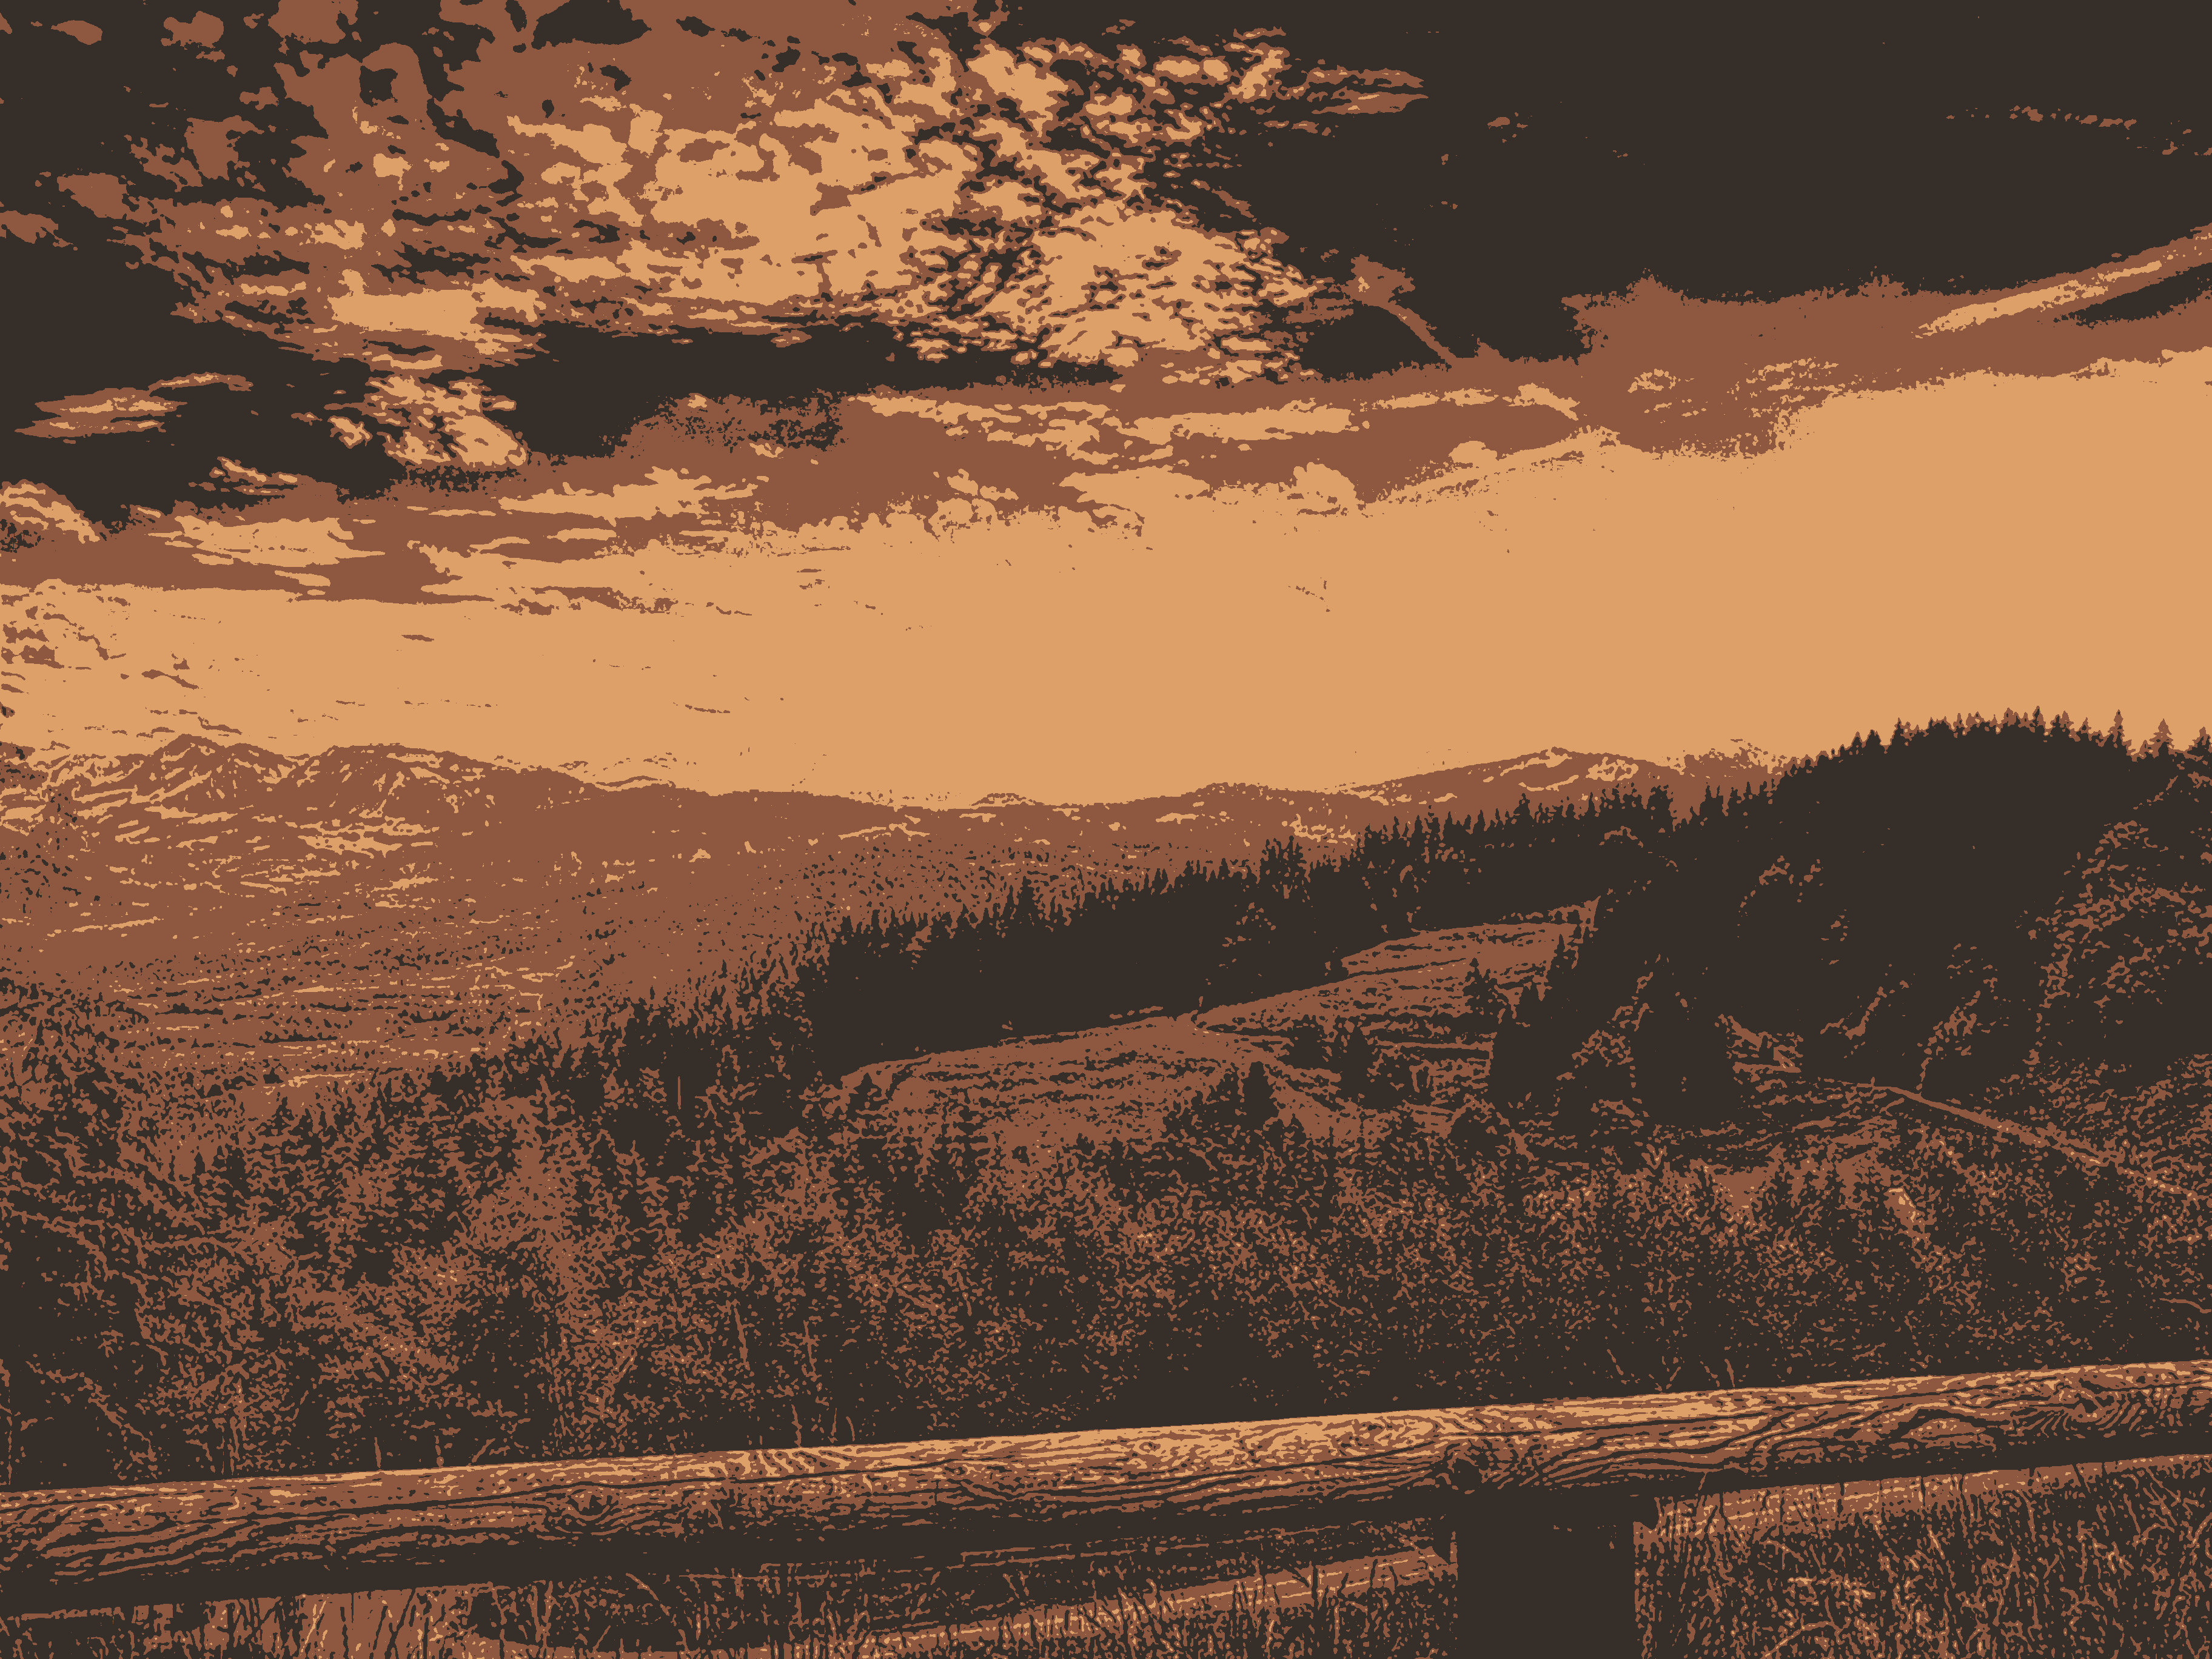
\includegraphics[width=0.45\textwidth]{imgs/output/k3_in_pixels.png}}
  \caption{Ảnh nén với \(k=3\)}
  \label{fig:k3}
\end{figure}

\begin{figure}[H]
  \centering
  \subfloat[random]{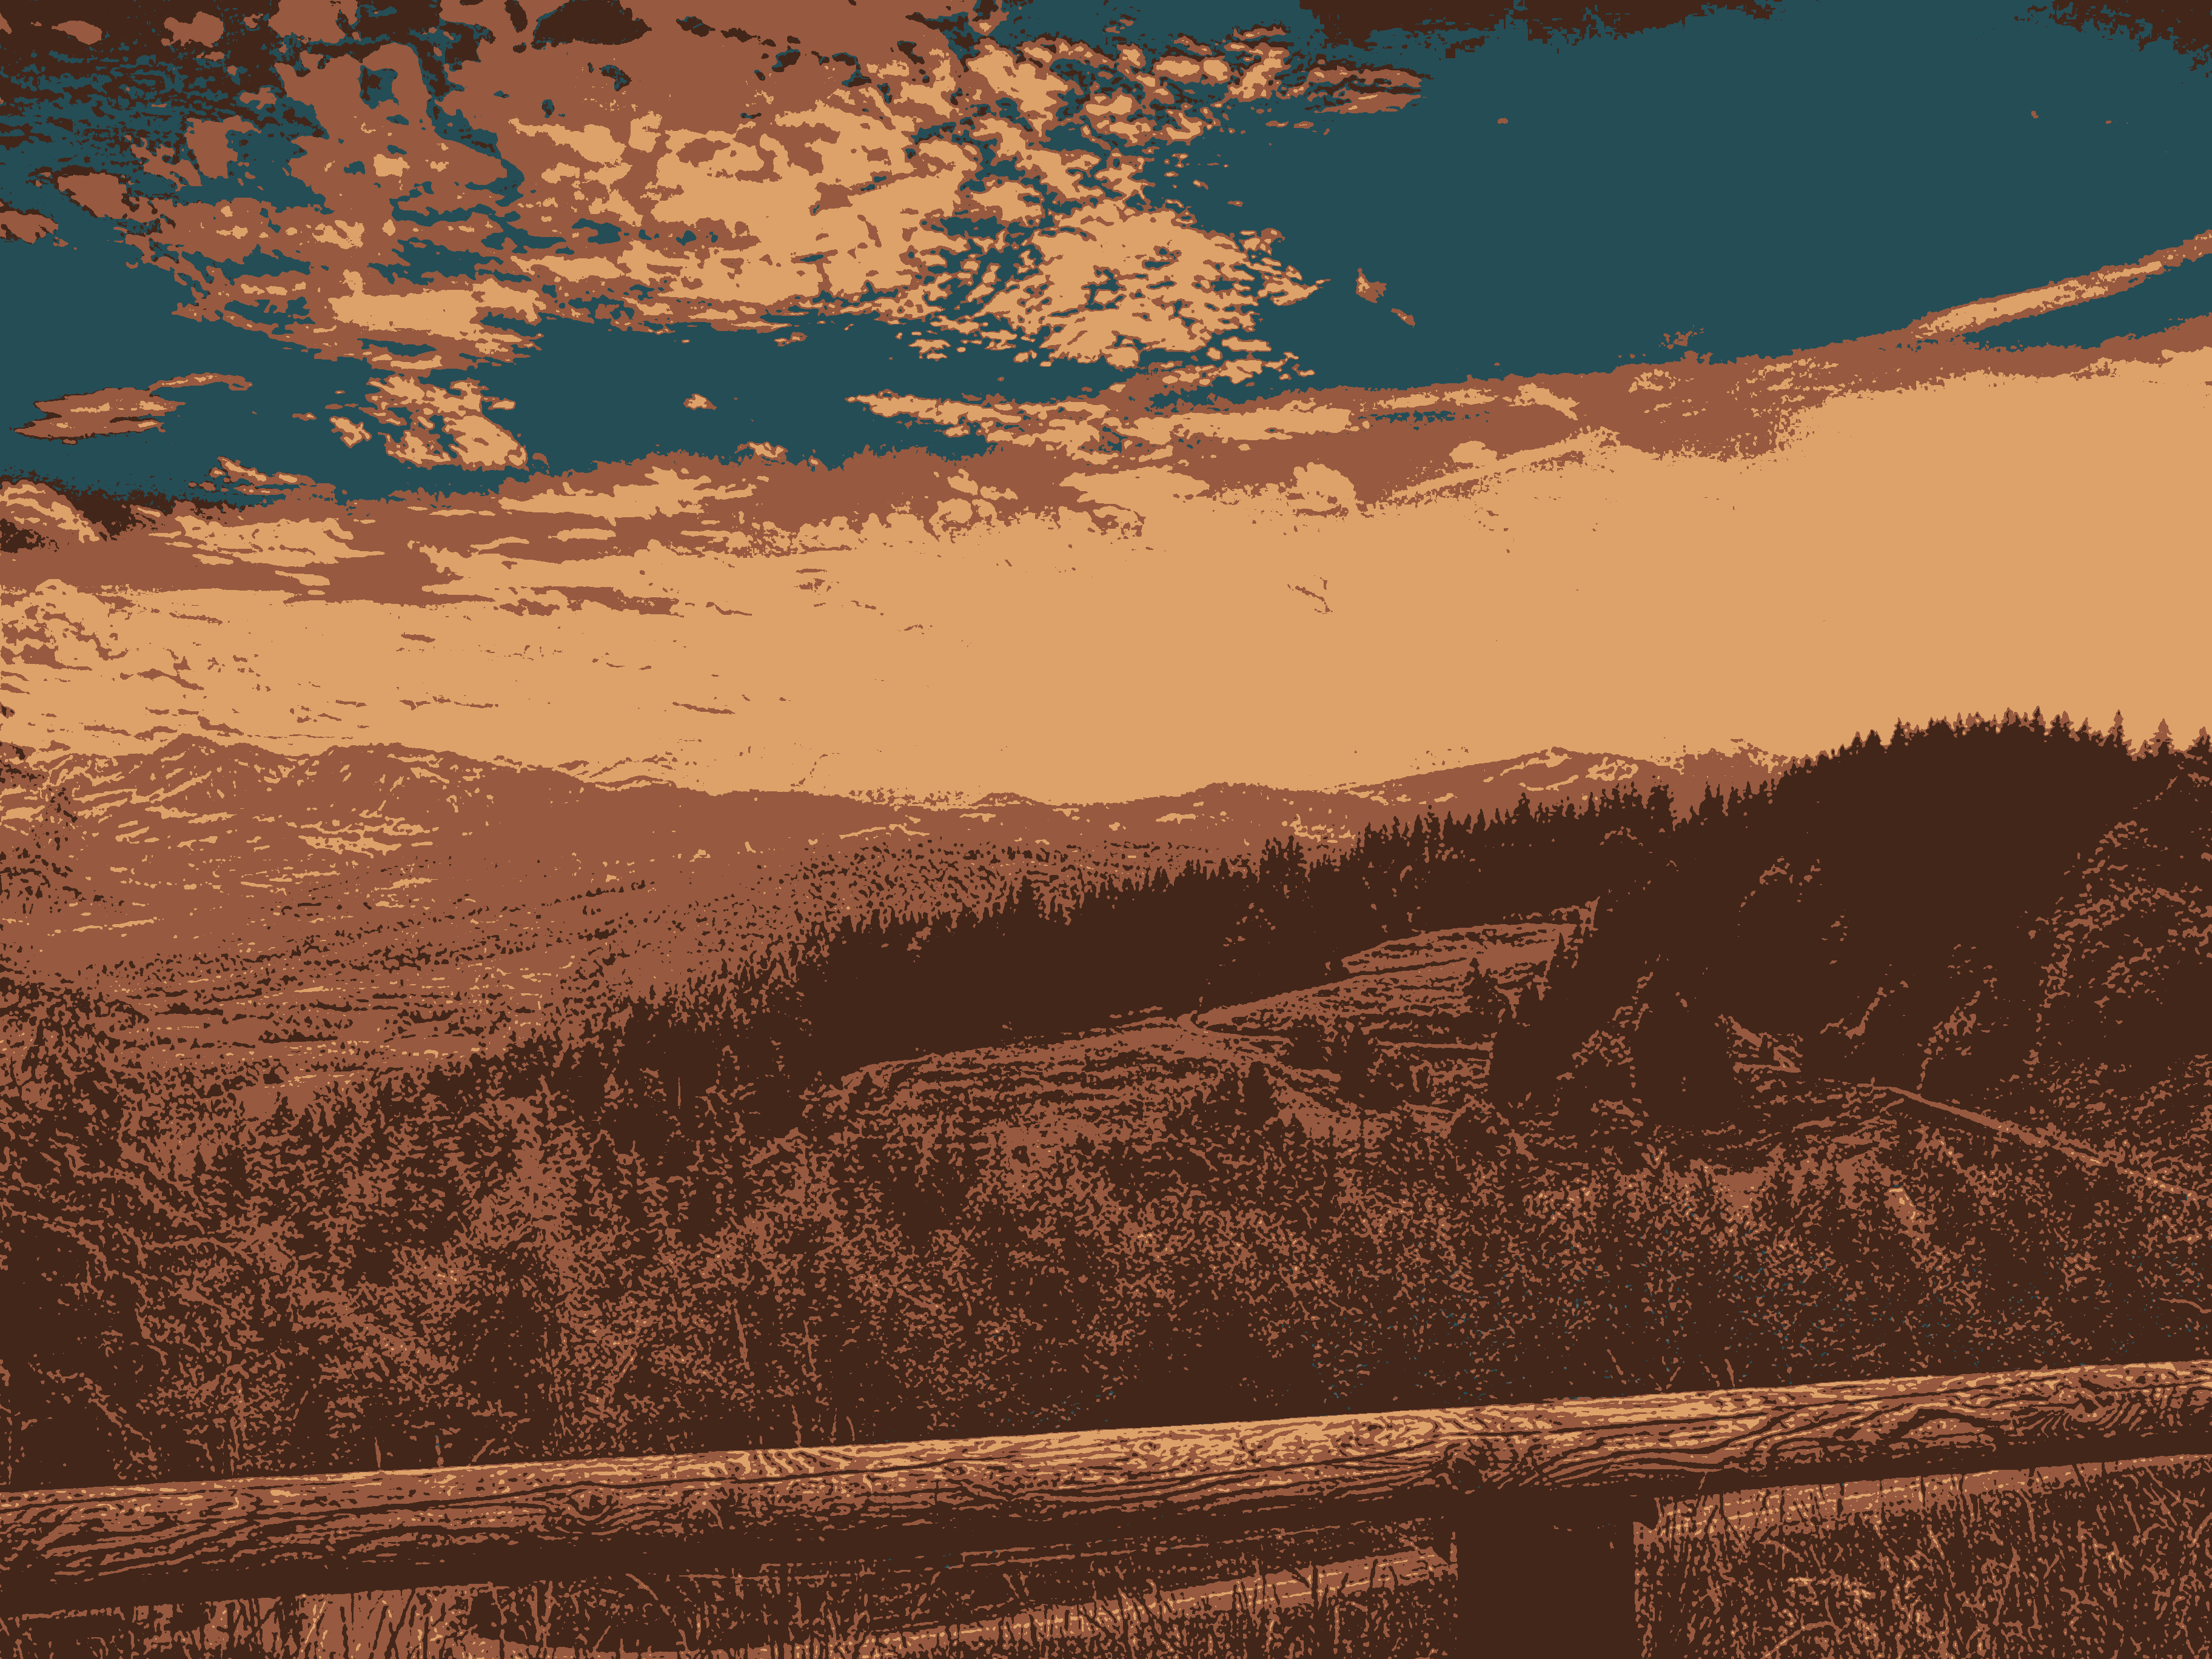
\includegraphics[width=0.45\textwidth]{imgs/output/k5_random.png}}
  \hfill
  \subfloat[in\_pixels]{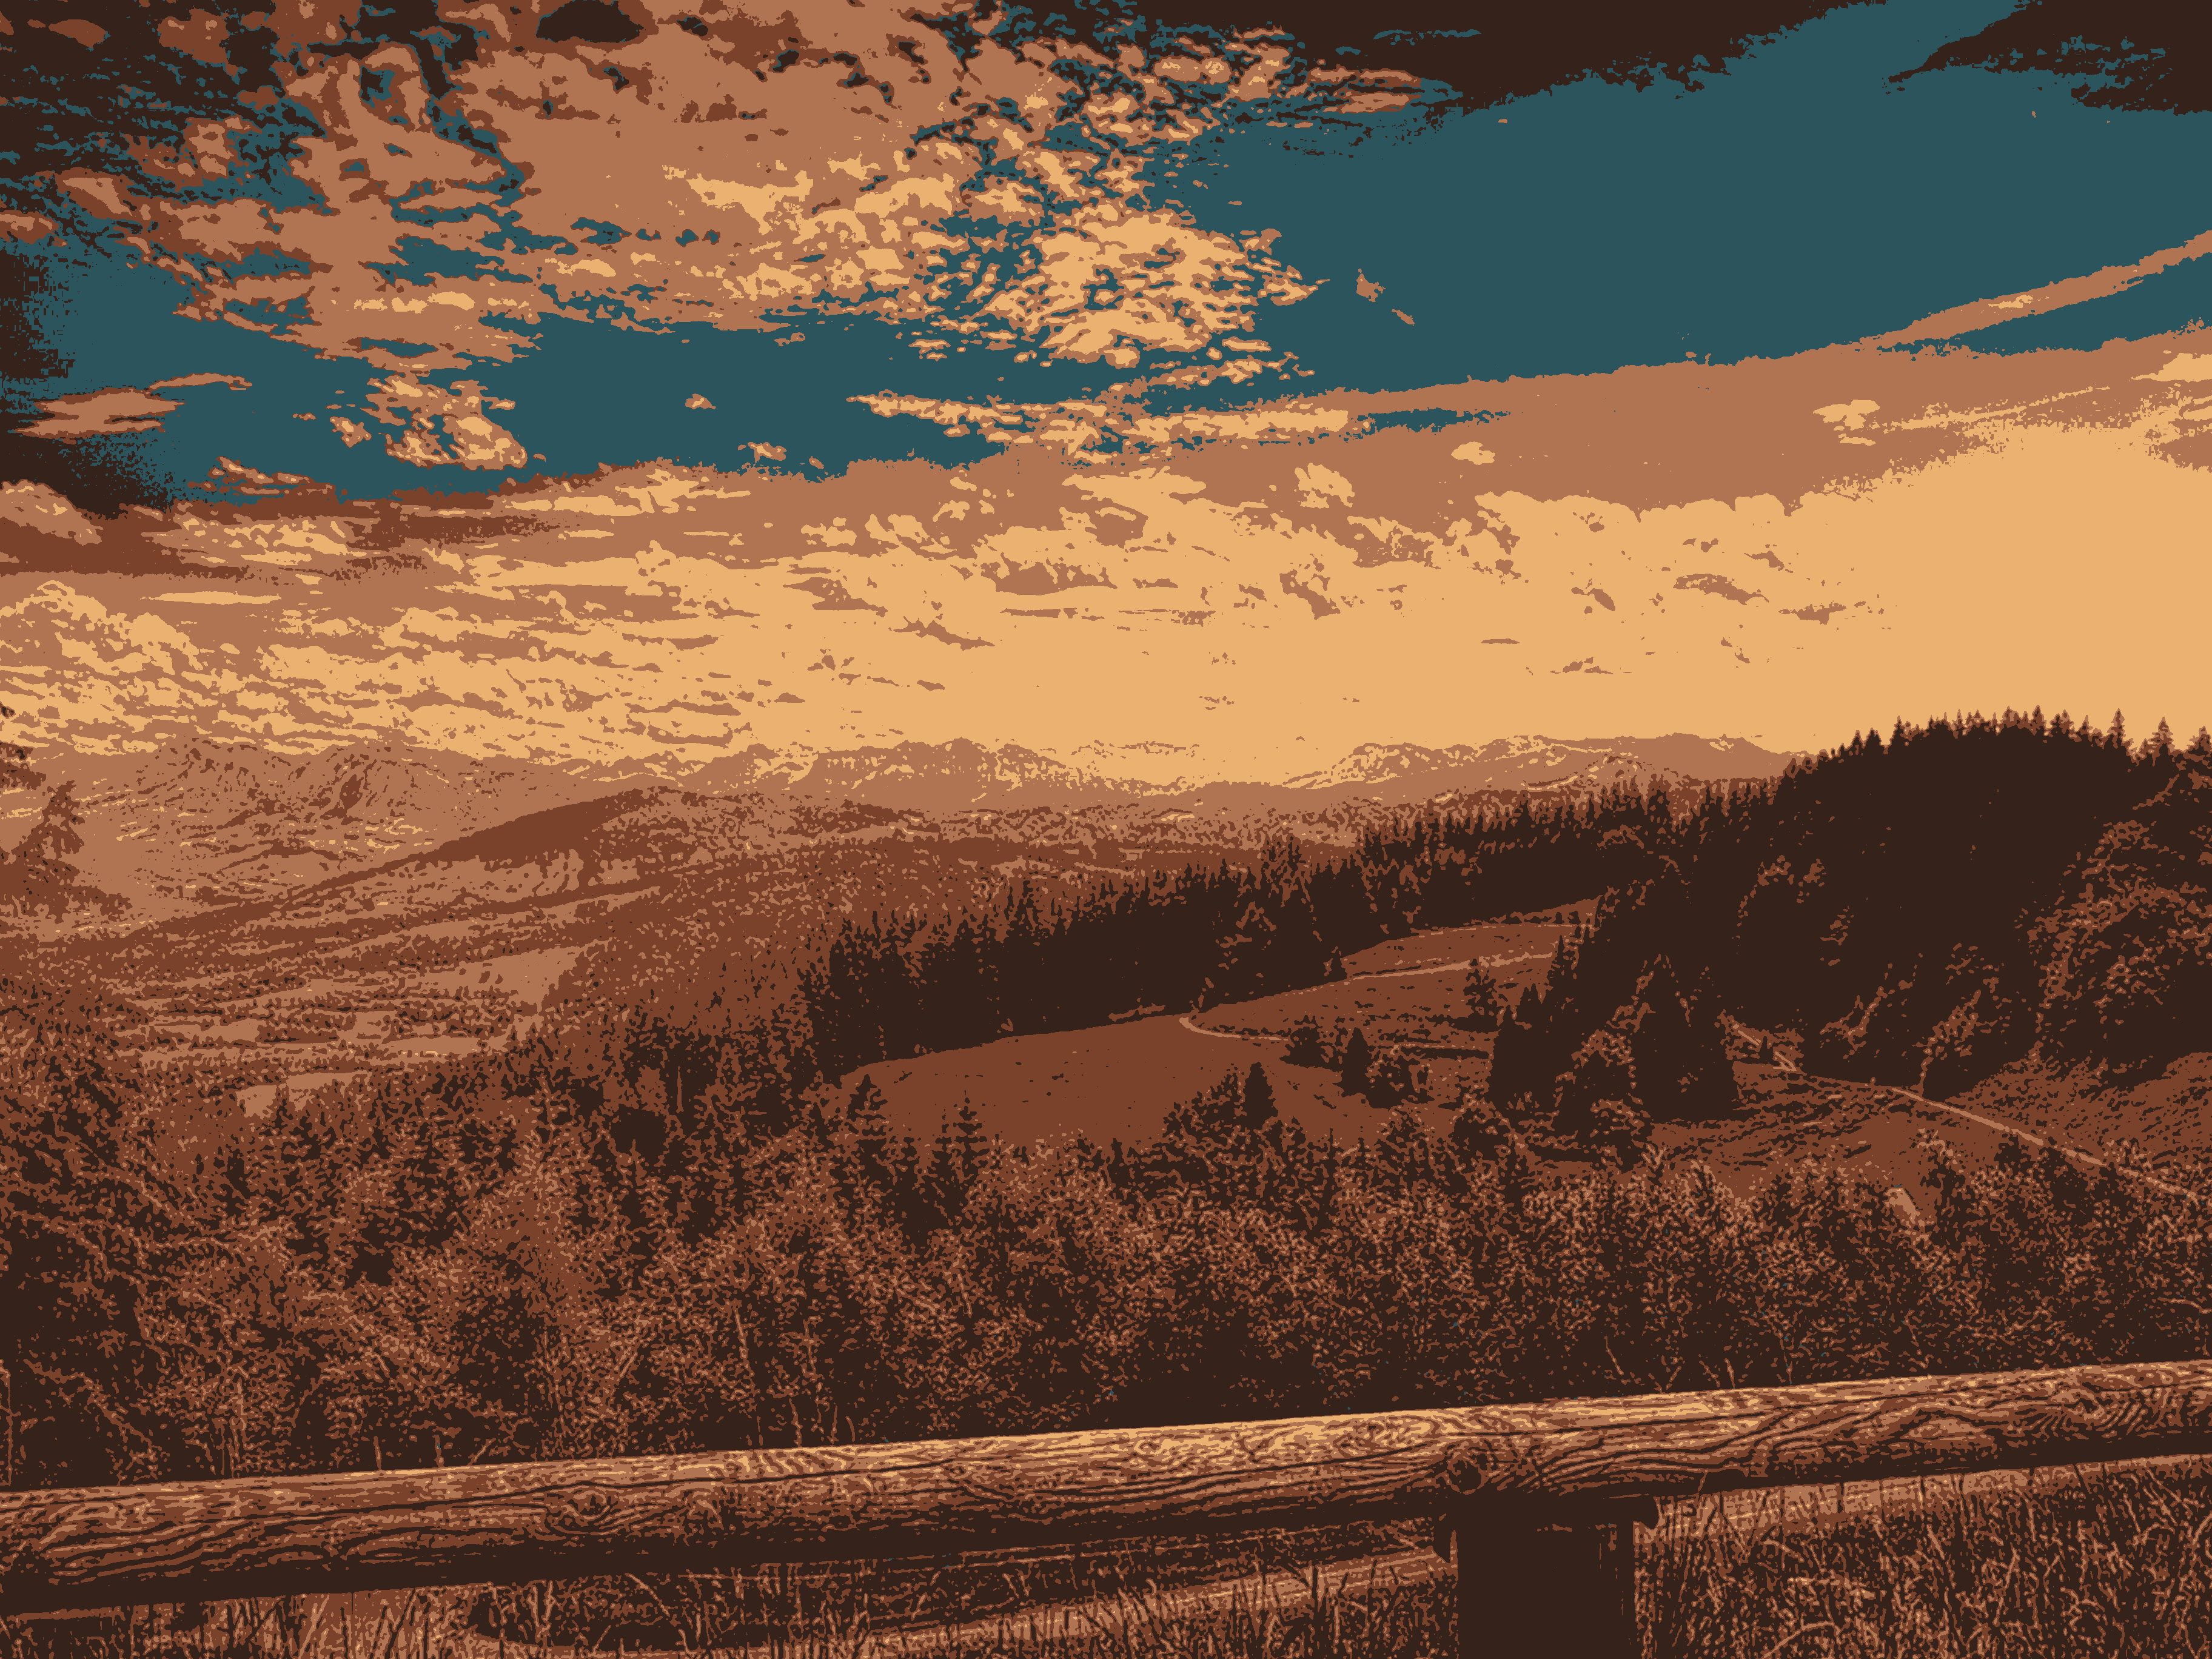
\includegraphics[width=0.45\textwidth]{imgs/output/k5_in_pixels.png}}
  \caption{Ảnh nén với \(k=5\)}
  \label{fig:k5}
\end{figure}

\begin{figure}[H]
  \centering
  \subfloat[random]{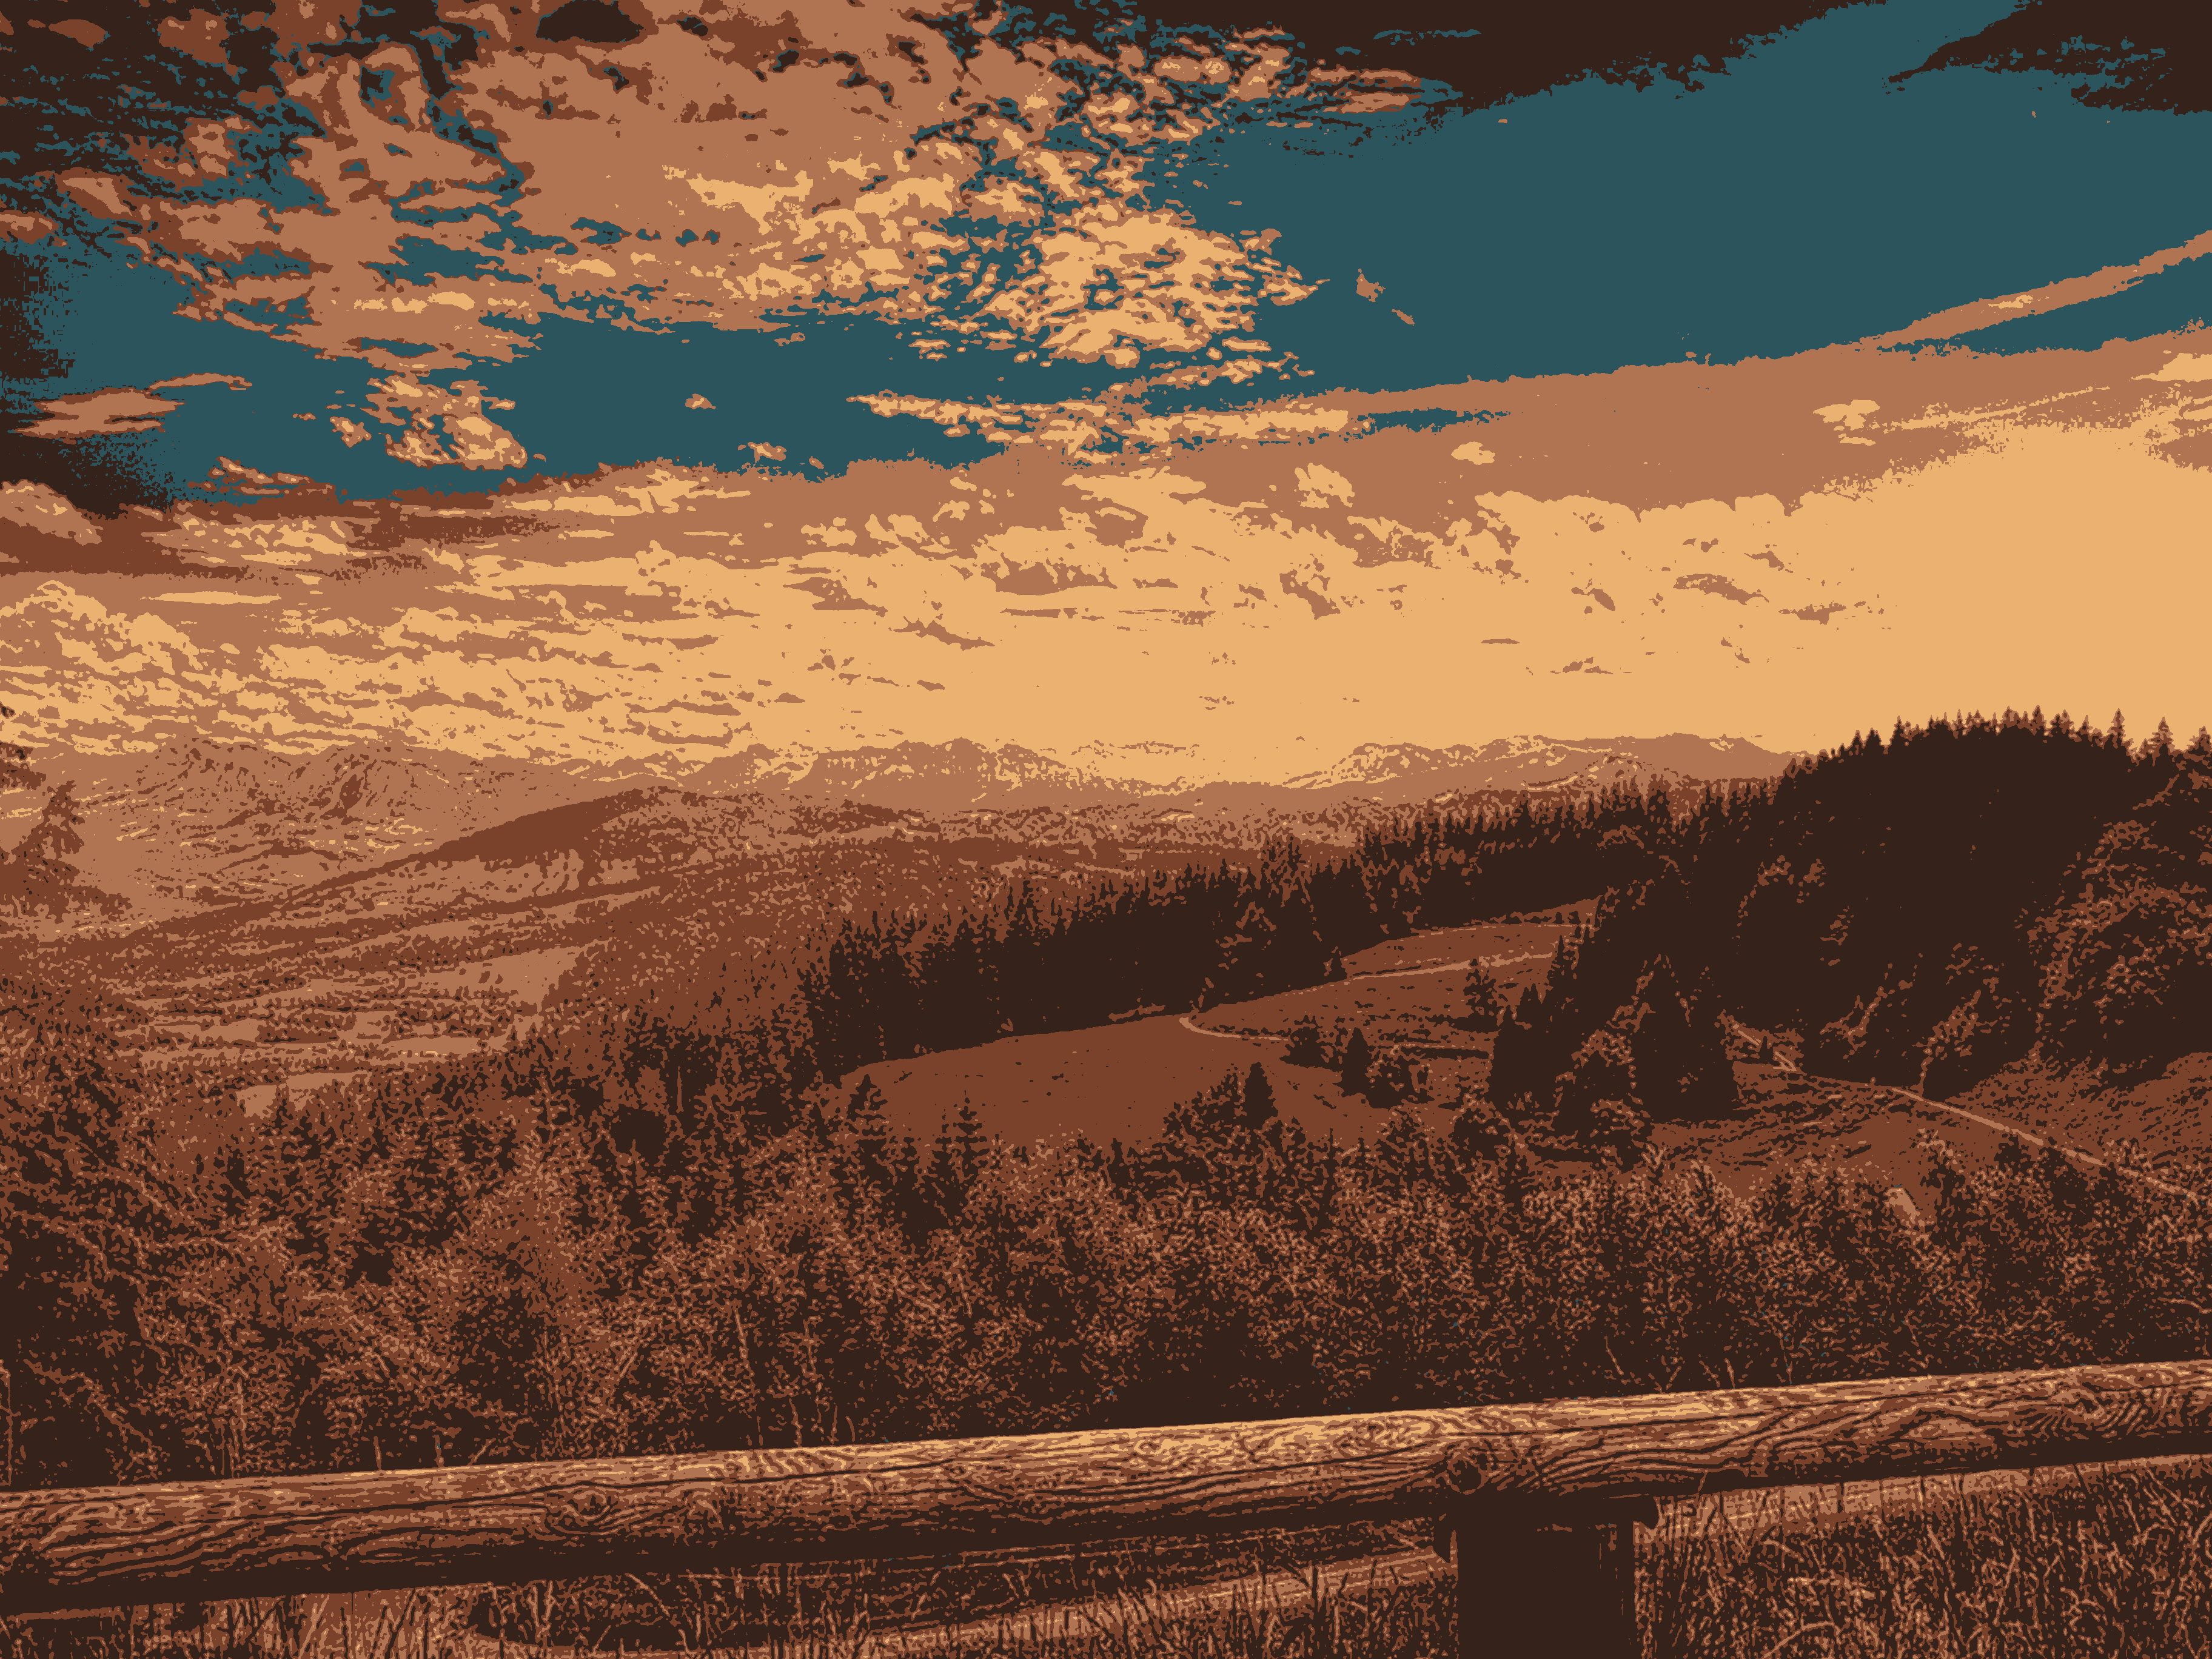
\includegraphics[width=0.45\textwidth]{imgs/output/k7_random.png}}
  \hfill
  \subfloat[in\_pixels]{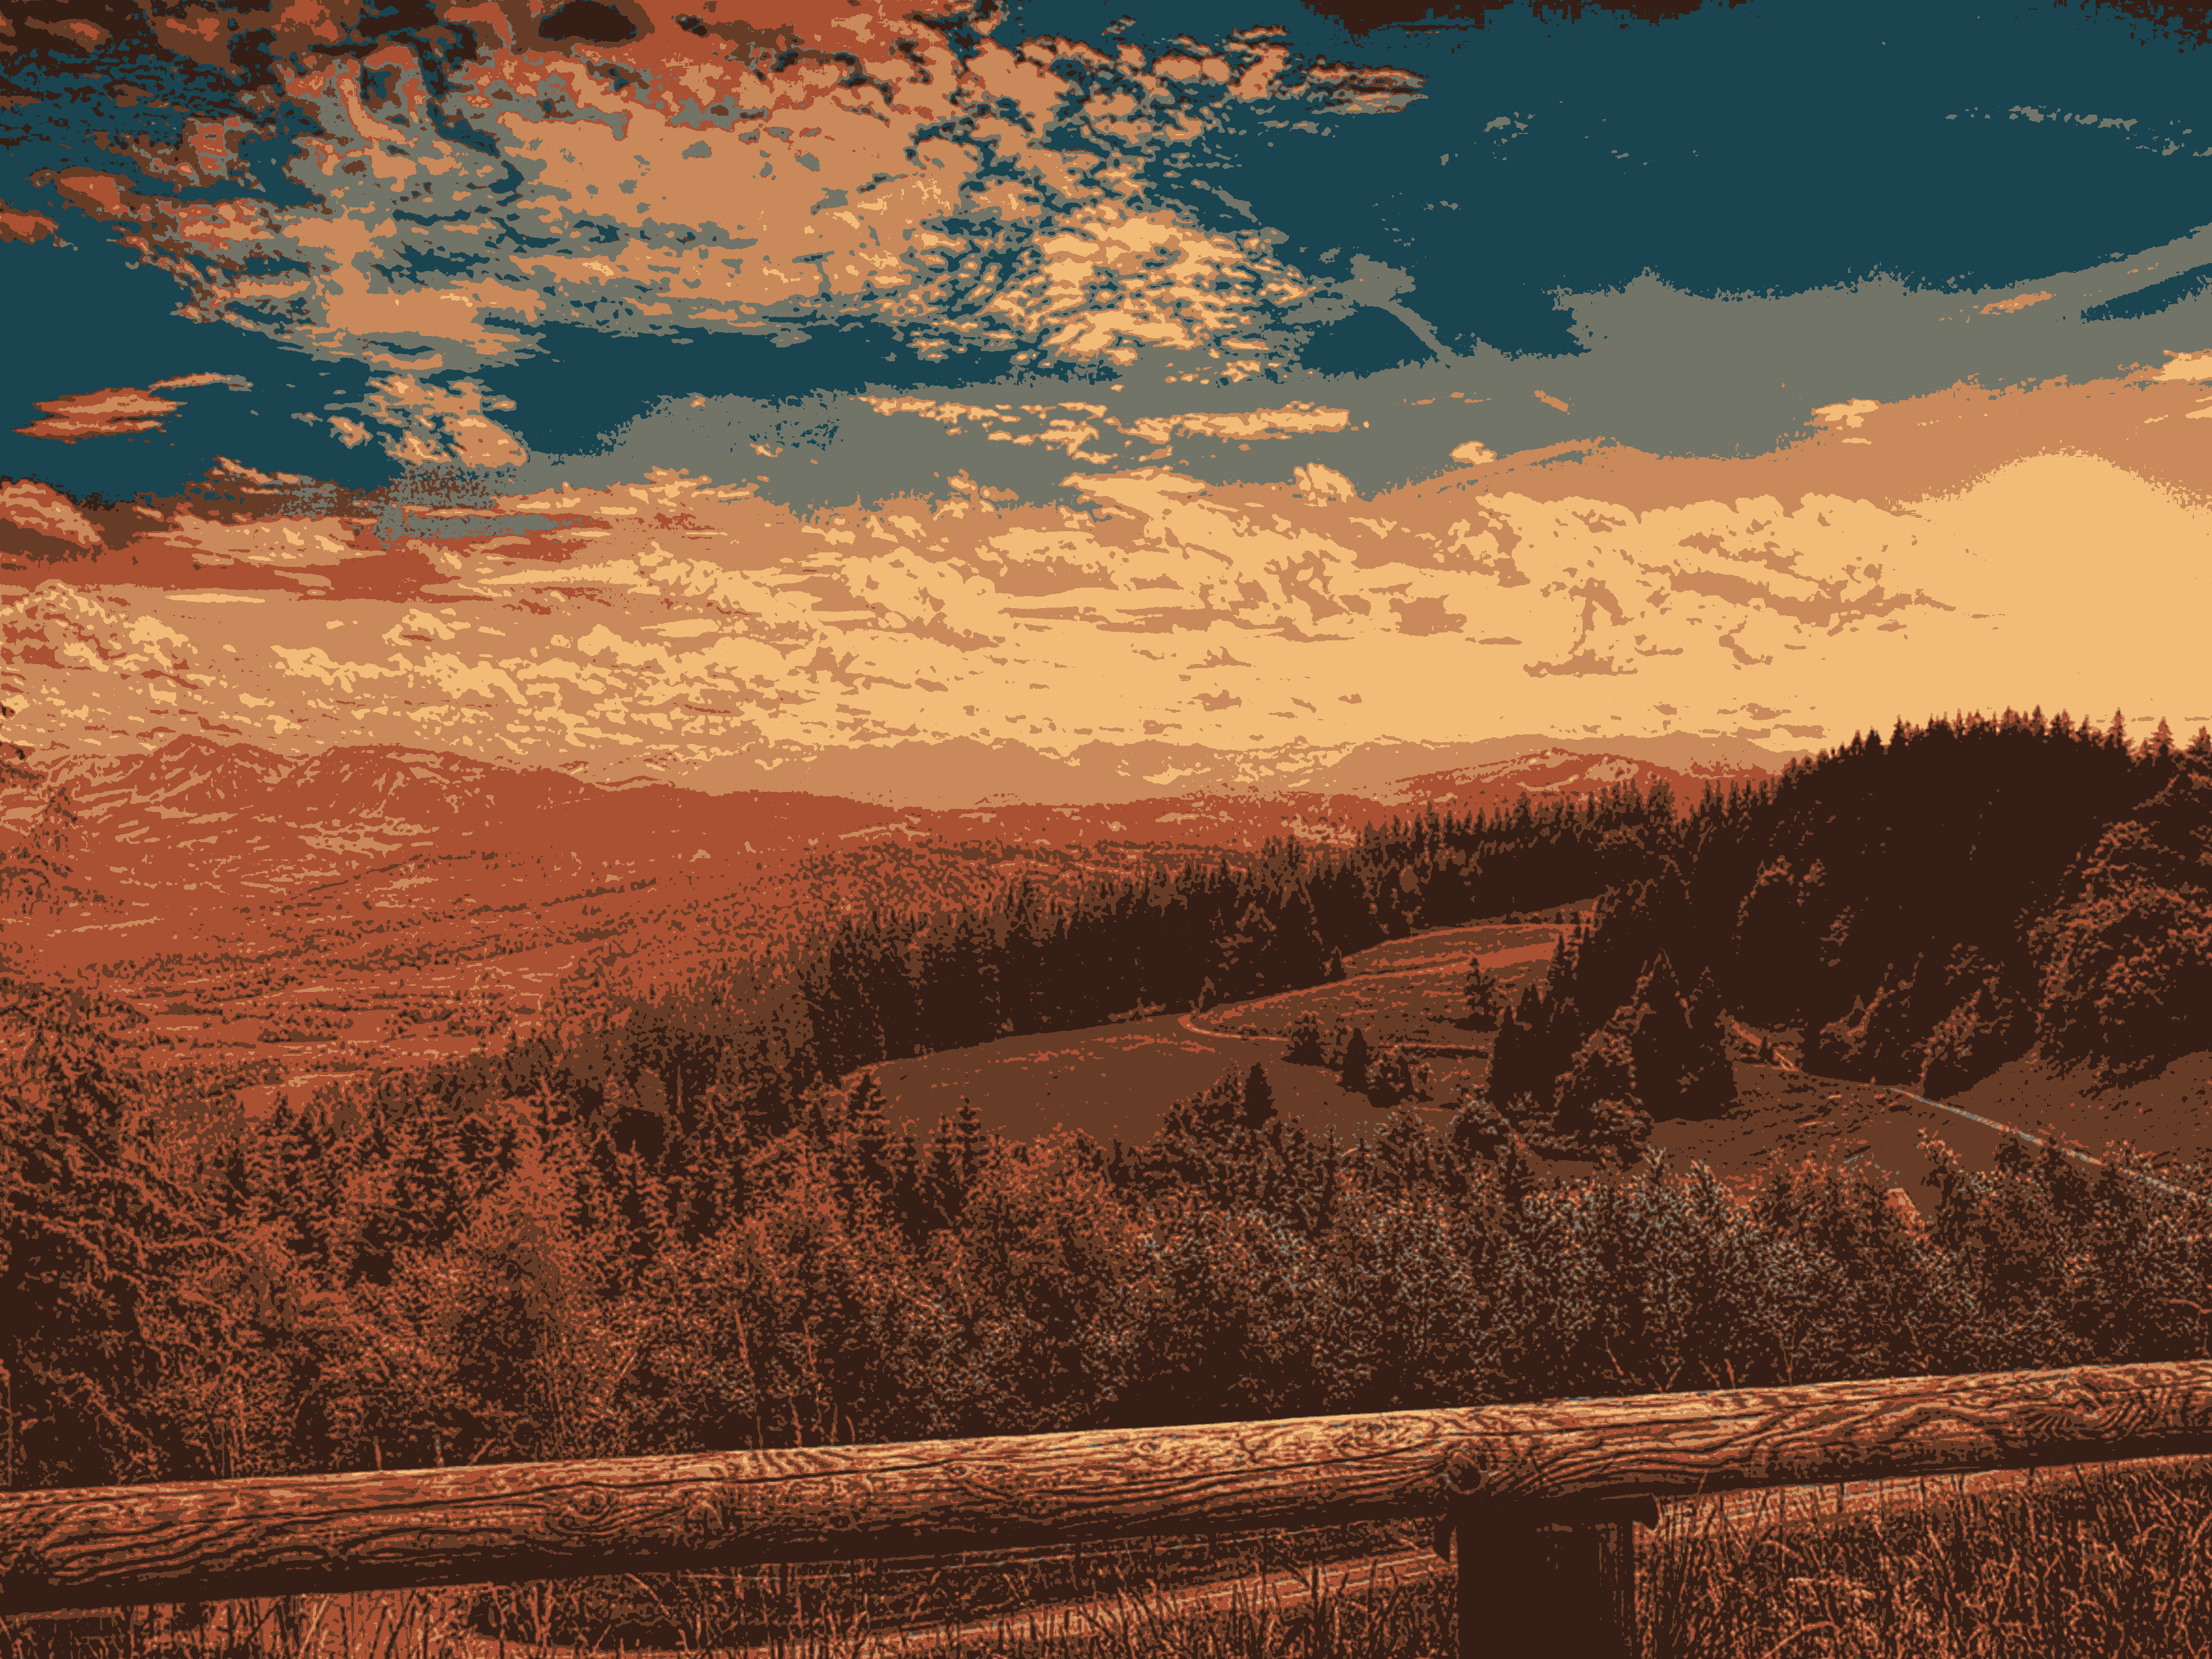
\includegraphics[width=0.45\textwidth]{imgs/output/k7_in_pixels.png}}
  \caption{Ảnh nén với \(k=7\)}
  \label{fig:k7}
\end{figure}

\begin{figure}[H]
  \centering
  \subfloat[random]{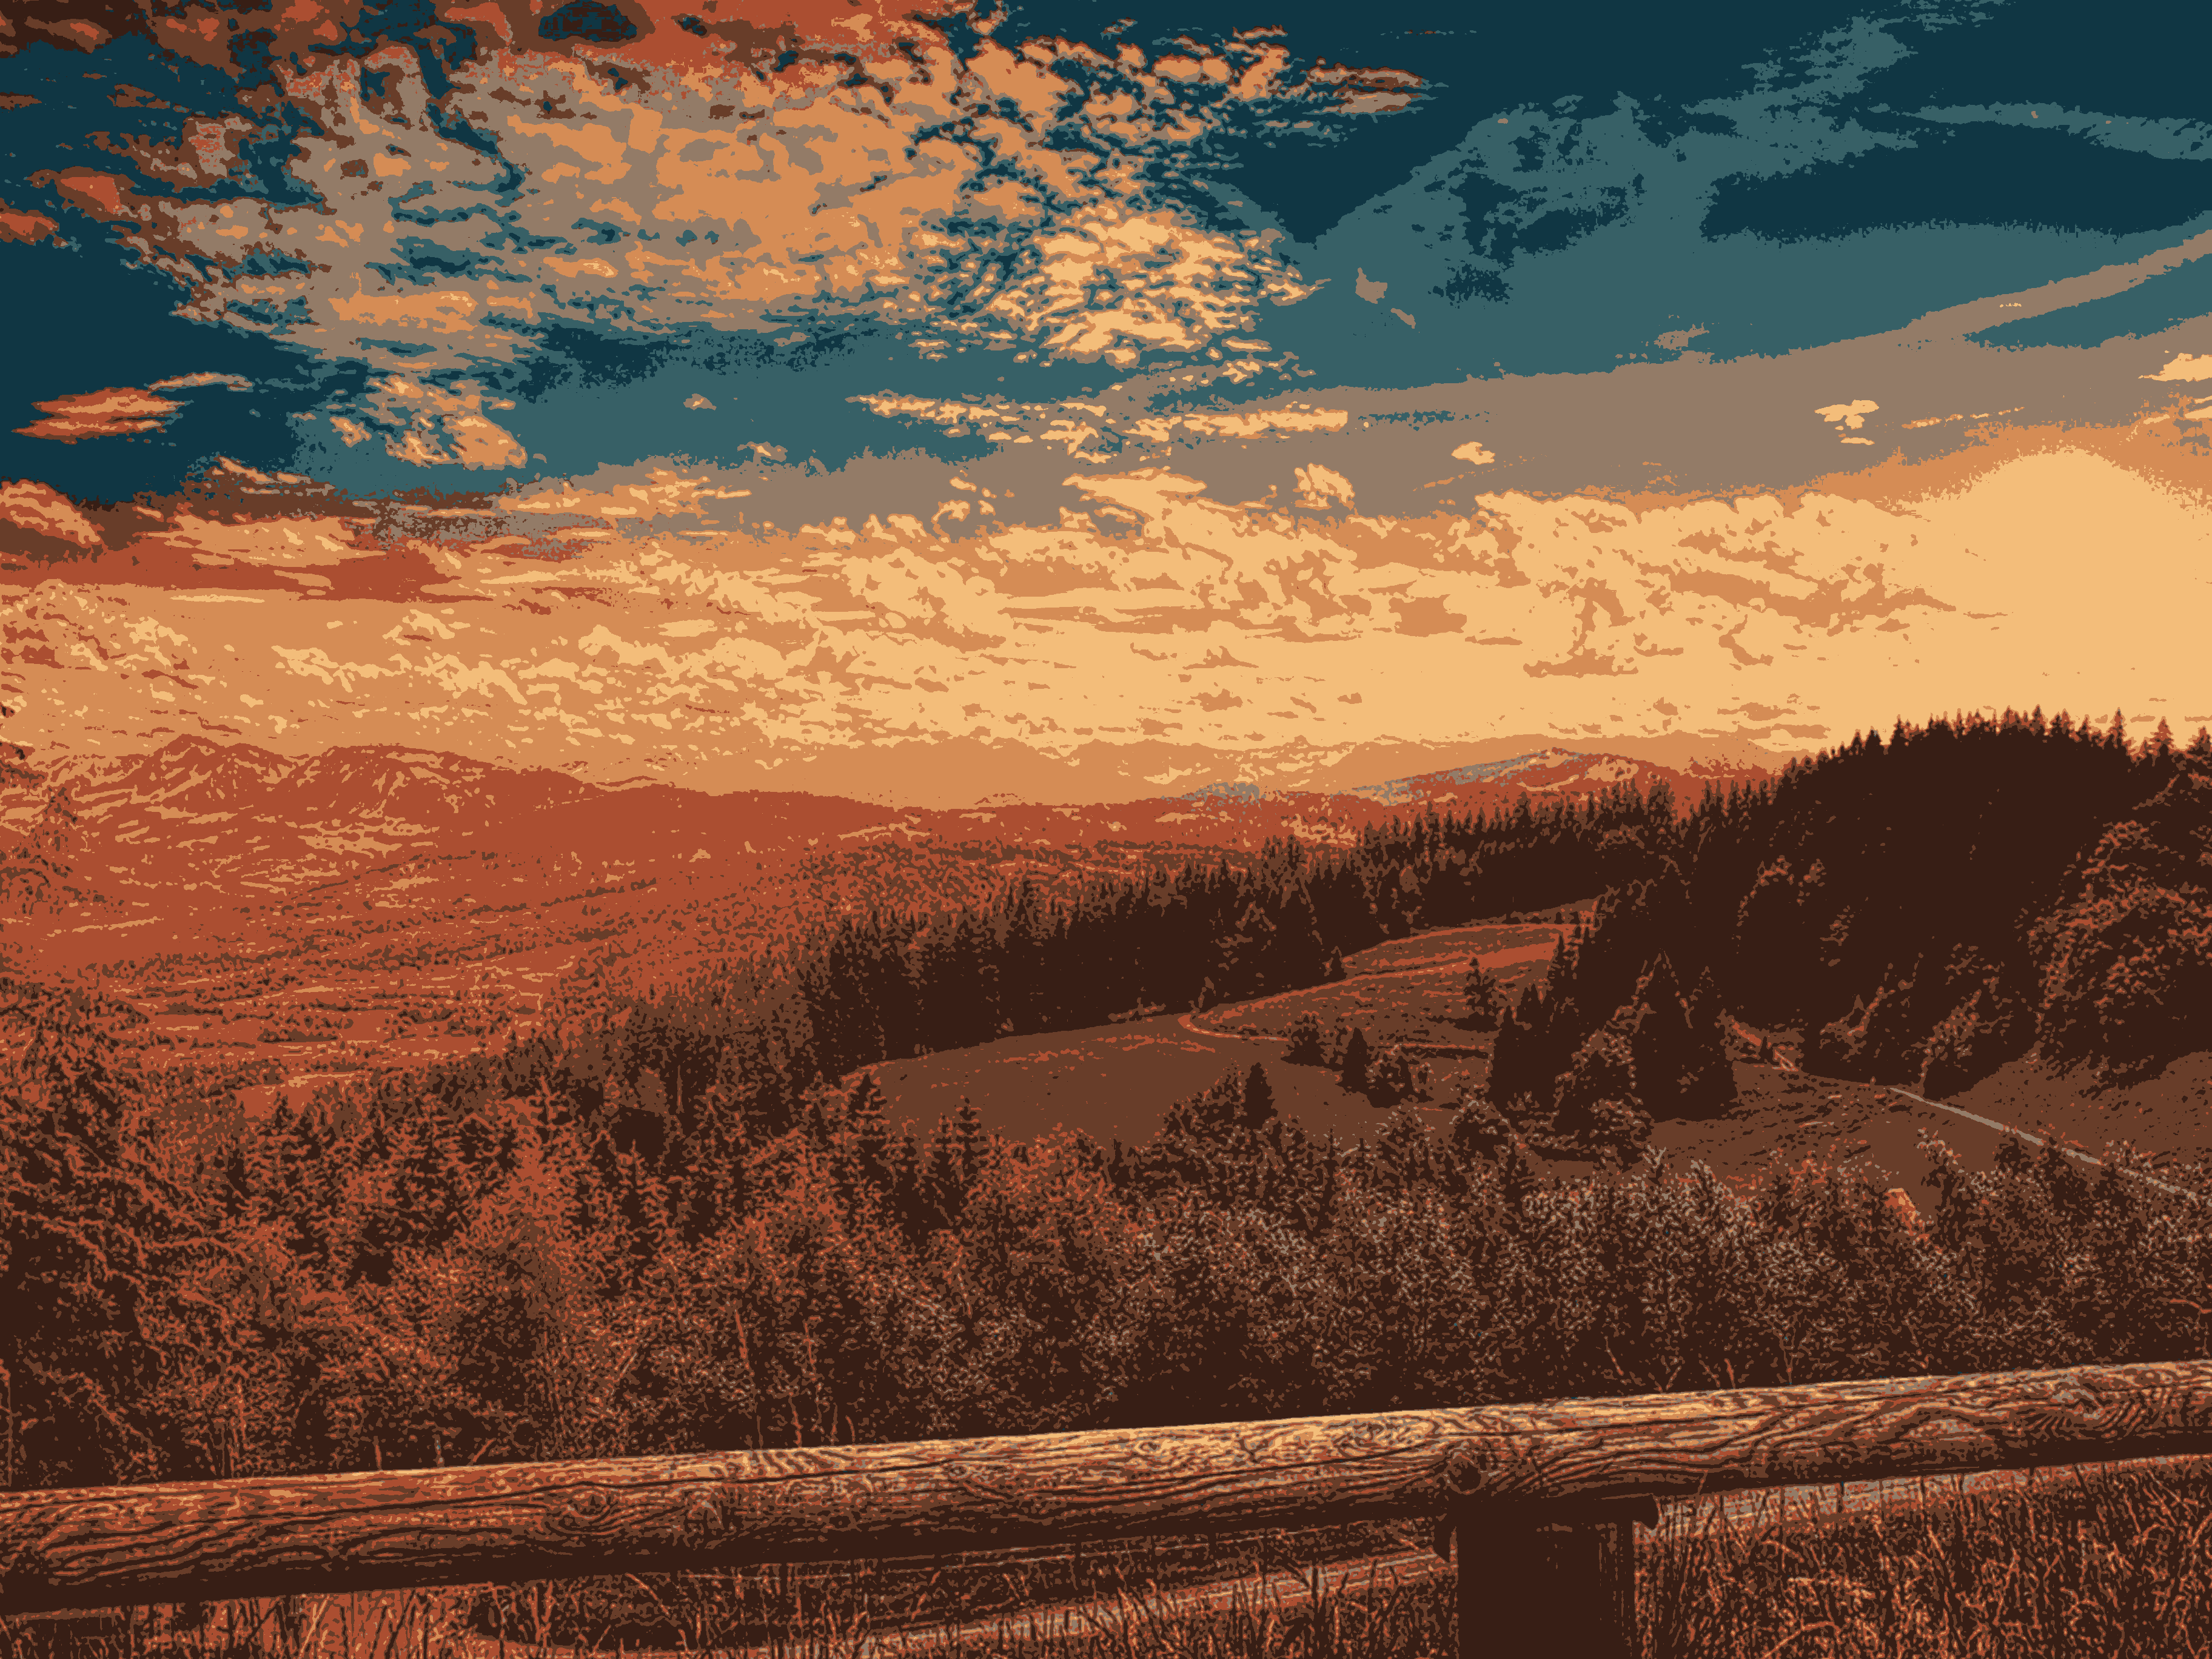
\includegraphics[width=0.45\textwidth]{imgs/output/k9_random.png}}
  \hfill
  \subfloat[in\_pixels]{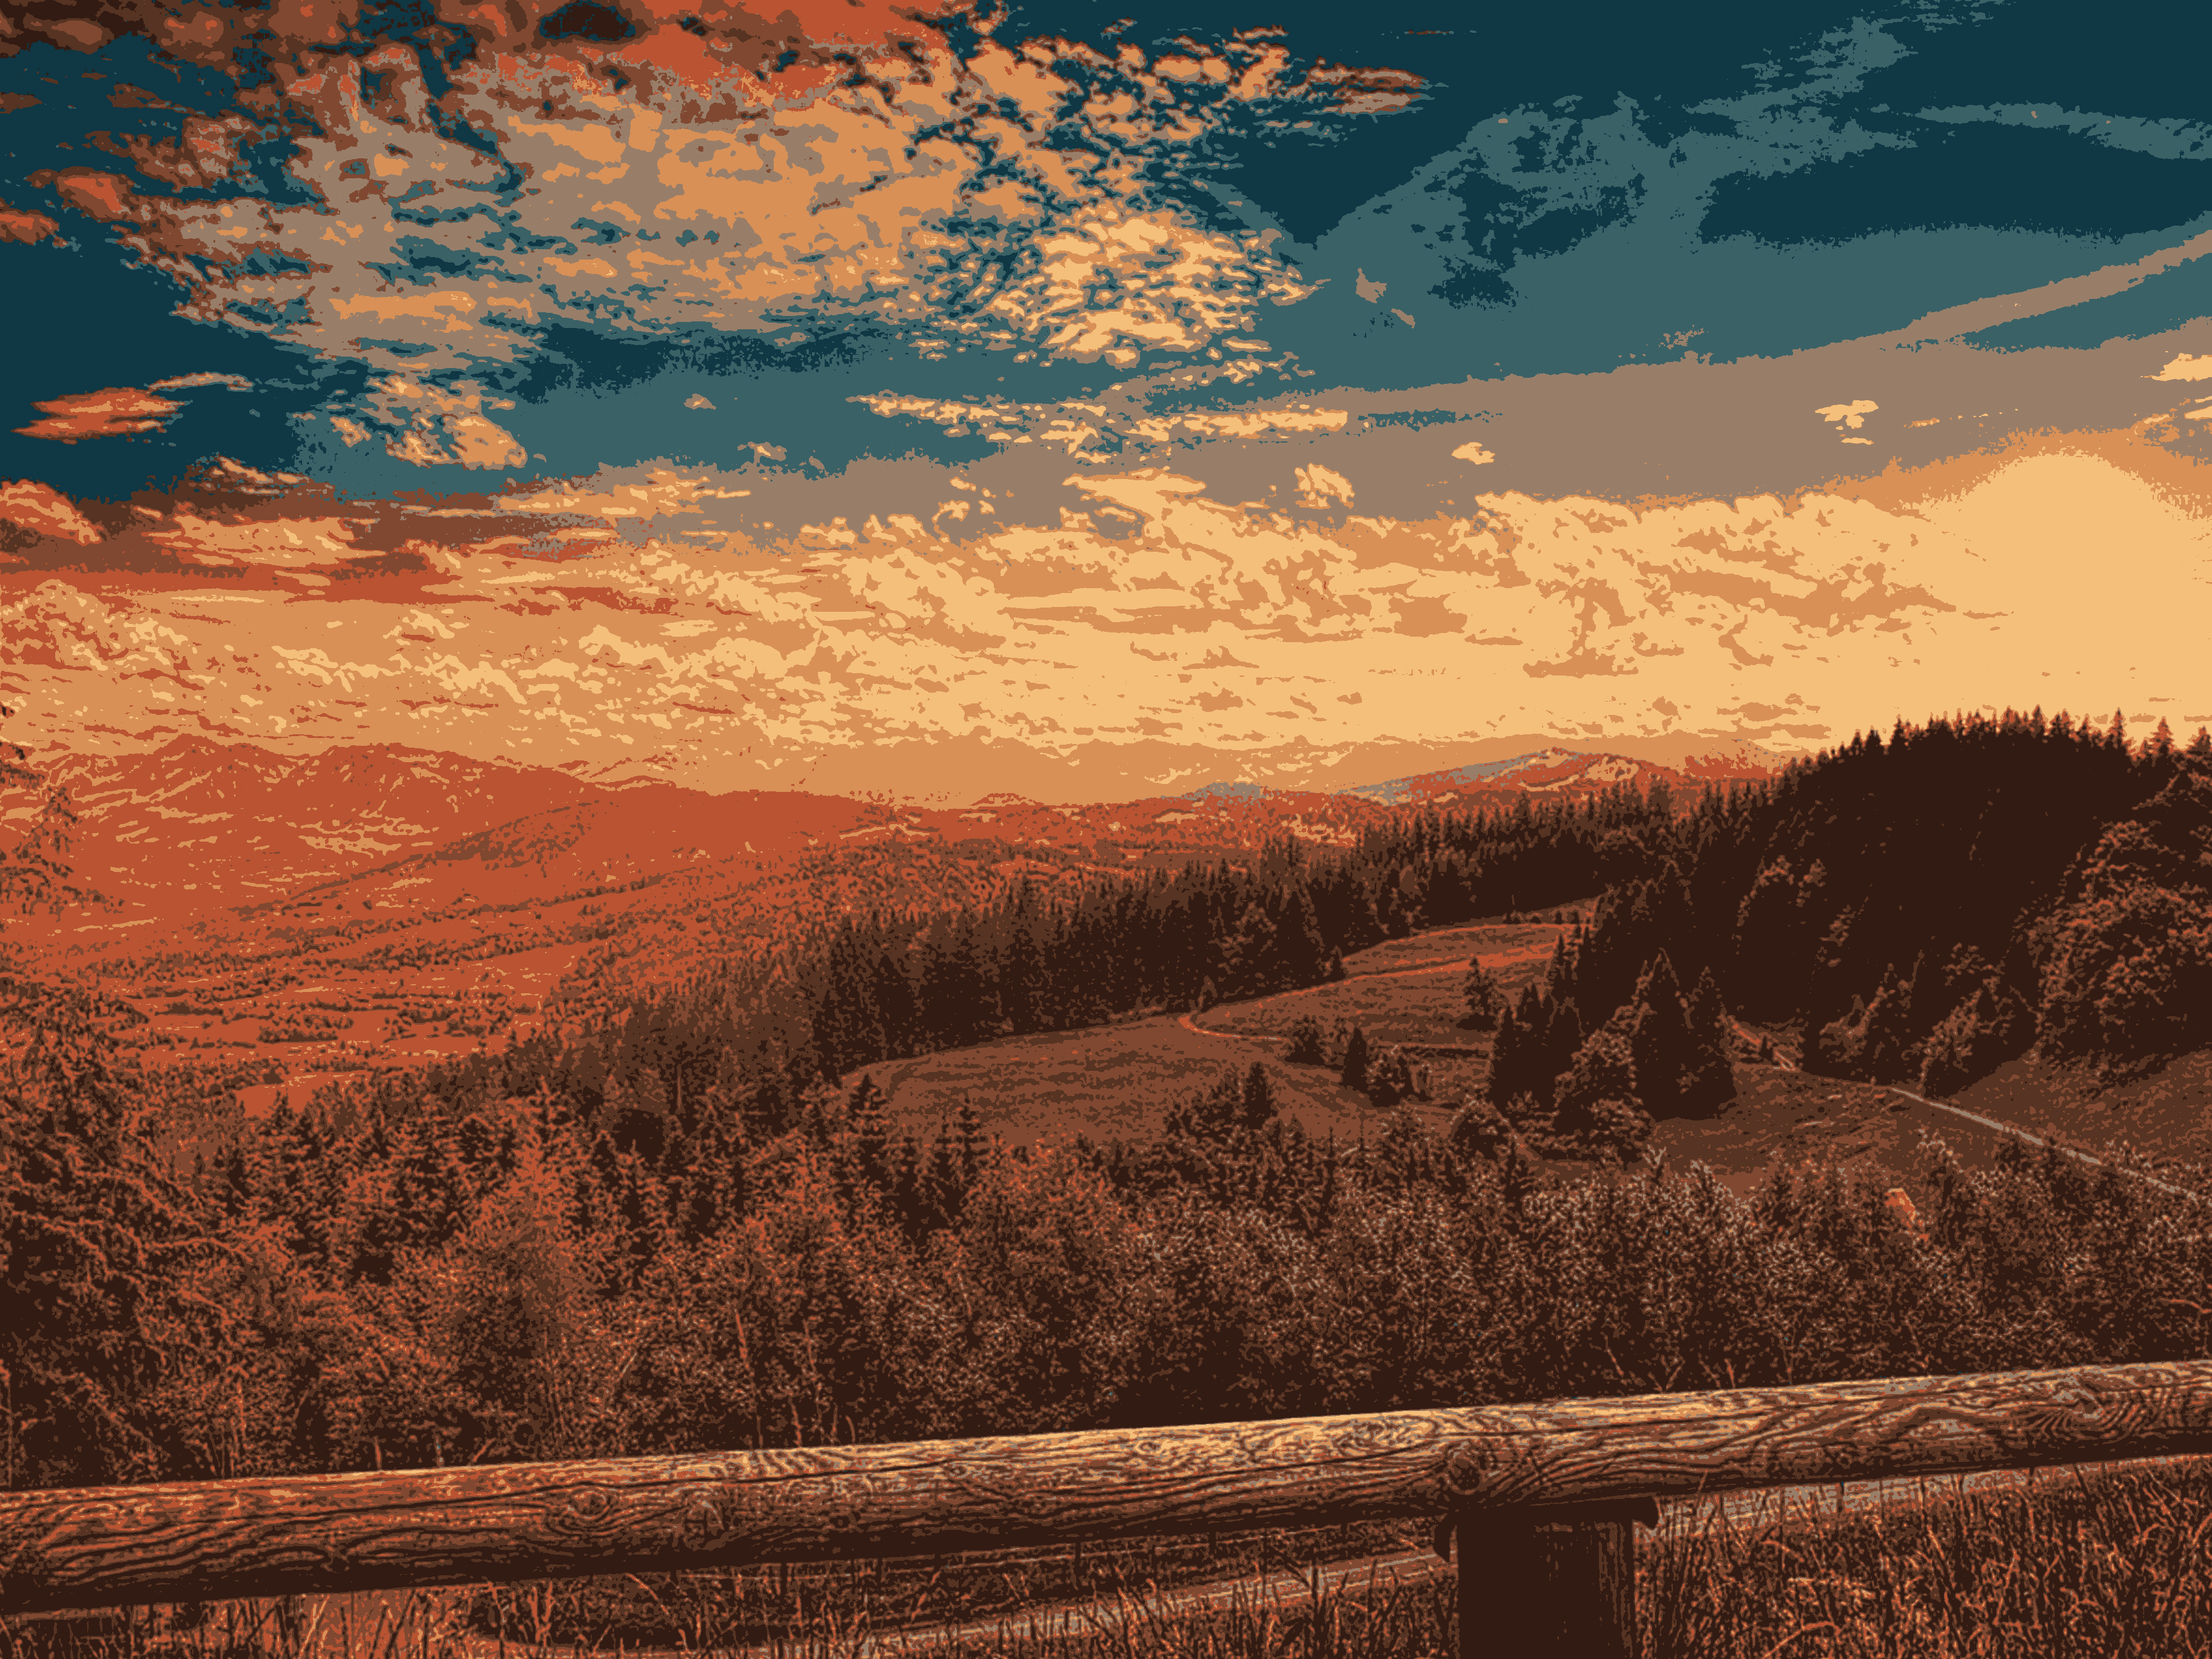
\includegraphics[width=0.45\textwidth]{imgs/output/k9_in_pixels.png}}
  \caption{Ảnh nén với \(k=9\)}
  \label{fig:k9}
\end{figure}

\newpage
\paragraph{Nhận xét chất lượng ảnh nén theo số màu}
\begin{itemize}
  \item \textbf{Với \(k=3\):} Ảnh chỉ giữ lại ba màu chủ đạo nên nhiều chi tiết nhỏ bị mất, đặc biệt ở các vùng chuyển màu. Tuy nhiên, các mảng màu lớn vẫn được phân biệt rõ và bố cục tổng thể của ảnh vẫn giữ nguyên.

  \item \textbf{Với \(k=5\):} Hình ảnh trở nên rõ ràng hơn, các gam màu phụ bắt đầu xuất hiện, giúp tái hiện các vùng chuyển tiếp màu và chi tiết nhỏ tốt hơn so với mức \(k=3\).

  \item \textbf{Với \(k=7\):} Ảnh gần như giữ lại đầy đủ các thông tin thị giác quan trọng. Các vùng chuyển tiếp màu mượt mà, giảm thiểu hiện tượng phân mảng màu, chất lượng hình ảnh tương đương với ảnh gốc về khả năng nhận diện.

  \item \textbf{Với \(k=9\):} Chất lượng tiếp tục được cải thiện nhẹ nhưng không quá khác biệt so với \(k=7\). Trong khi đó, chi phí tính toán tiếp tục tăng, cho thấy \(k=7\) đã là mức tối ưu cho bài toán này.
\end{itemize}

Ngoài ra, so sánh giữa hai phương pháp khởi tạo centroid:
\begin{itemize}
  \item \textit{in\_pixels} có xu hướng tái hiện màu trung thực hơn ở các mức \(k\) thấp do chọn trực tiếp các giá trị từ pixel thực tế.
  \item \textit{random} đôi khi gây sai lệch nhẹ về màu sắc ở mức \(k\) thấp, nhưng khi \(k\) tăng, sự khác biệt giữa hai phương pháp này dần thu hẹp và kết quả gần tương đồng.
\end{itemize}

\paragraph{Kết luận:}
Chất lượng ảnh nén tăng rõ rệt theo số cụm màu \(k\), nhưng từ \(k=7\) trở đi, sự cải thiện thị giác không còn nhiều trong khi thời gian tính toán tăng đáng kể. Do đó, giá trị \(k=7\) được xem là hợp lý nhất cho bài toán nén màu ảnh RGB kích thước trung bình.

\newpage
\subsection{Thời gian thực thi}

Kết quả benchmark cho thấy thời gian thực thi của thuật toán \(k\)-means chịu ảnh hưởng trực tiếp bởi hai tham số chính: số cụm \(k\) và số vòng lặp tối đa \texttt{max\_iter}.

\begin{itemize}
  \item Khi tăng số cụm \(k\), số lượng phép tính khoảng cách và cập nhật centroid ở mỗi vòng lặp tăng lên, dẫn đến thời gian thực thi dài hơn.
  \item Khi tăng \texttt{max\_iter}, nếu thuật toán chưa hội tụ sớm, tổng số vòng lặp thực hiện sẽ nhiều hơn, làm tăng thời gian xử lý.
\end{itemize}

\textbf{Ảnh hưởng của \texttt{max\_iter}} được thể hiện trong Hình~\ref{fig:runtime_maxiter}. Dễ thấy rằng thời gian thực thi tăng dần khi \texttt{max\_iter} tăng từ 20 lên 200, đặc biệt rõ rệt khi số cụm \(k\) lớn.

\begin{figure}[H]
  \centering
  \subfloat[\texttt{max\_iter} = 20]{%
    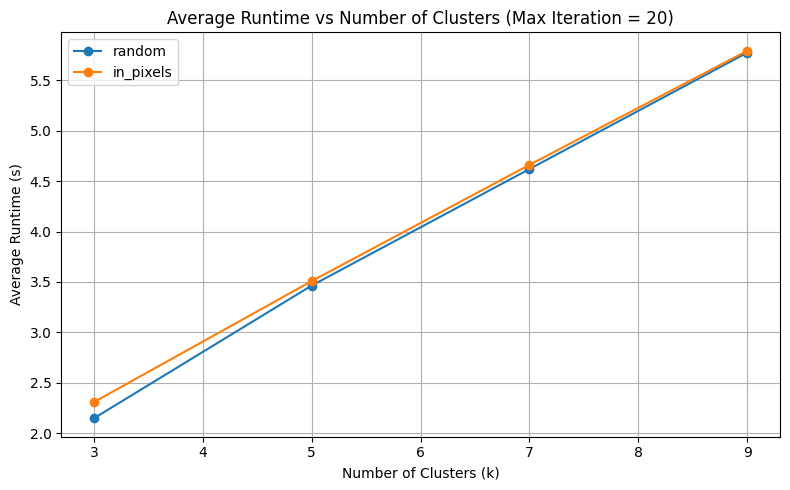
\includegraphics[width=0.48\linewidth]{imgs/benchmark/maxiter20.png}
  }
  \hfill
  \subfloat[\texttt{max\_iter} = 50]{%
    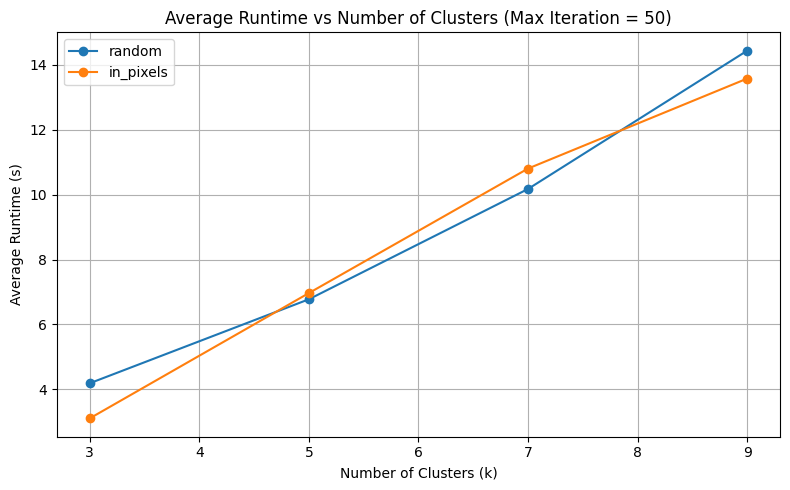
\includegraphics[width=0.48\linewidth]{imgs/benchmark/maxiter50.png}
  }

  \subfloat[\texttt{max\_iter} = 100]{%
    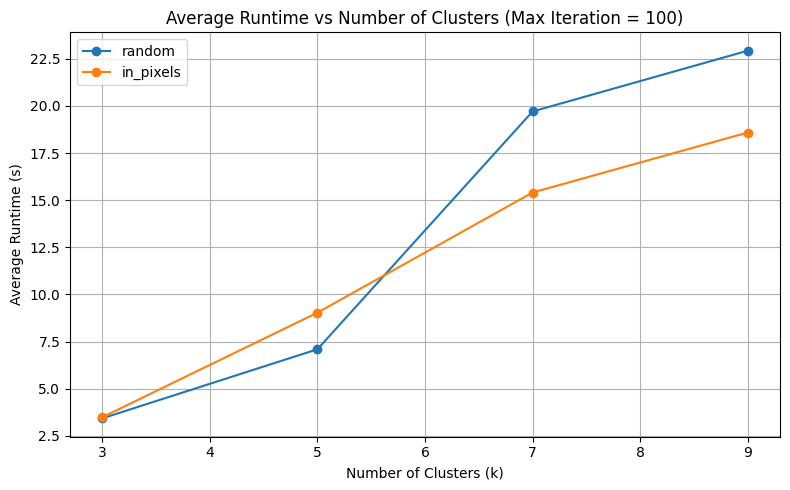
\includegraphics[width=0.48\linewidth]{imgs/benchmark/maxiter100.png}
  }
  \hfill
  \subfloat[\texttt{max\_iter} = 200]{%
    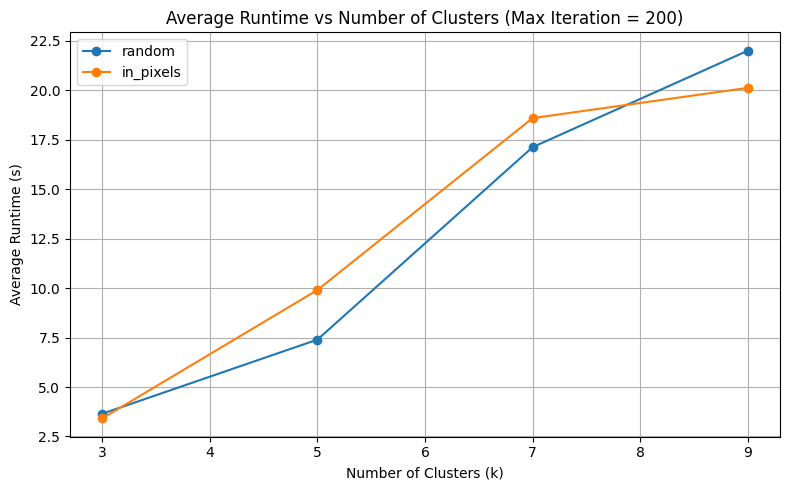
\includegraphics[width=0.48\linewidth]{imgs/benchmark/maxiter200.png}
  }
  \caption{Thời gian thực thi trung bình với các giá trị \texttt{max\_iter} khác nhau}
  \label{fig:runtime_maxiter}
\end{figure}

\textbf{Ảnh hưởng của số cụm \(k\)} được thể hiện rõ qua Hình~\ref{fig:runtime_k}. Khi tăng từ 3 lên 9 cụm, thời gian xử lý tăng gần tuyến tính, do mỗi vòng lặp cần tính nhiều khoảng cách hơn và quá trình cập nhật centroid cũng phức tạp hơn.

\begin{figure}[H]
  \centering
  \subfloat[\(k = 3\)]{%
    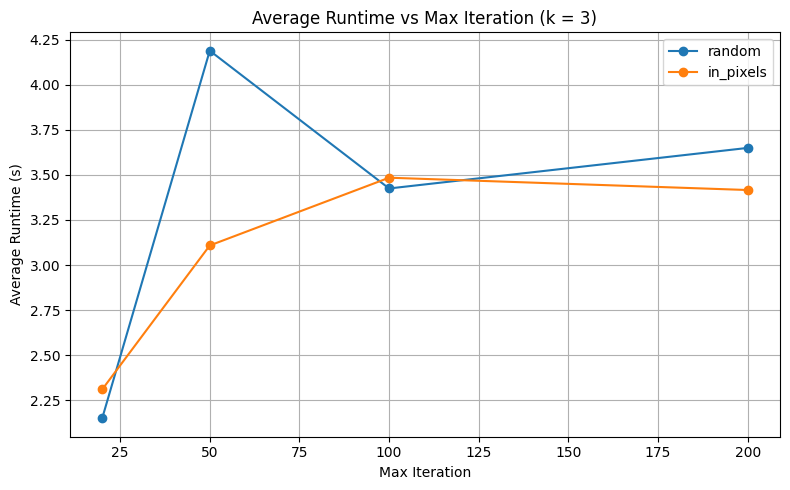
\includegraphics[width=0.48\linewidth]{imgs/benchmark/k3.png}
  }
  \hfill
  \subfloat[\(k = 5\)]{%
    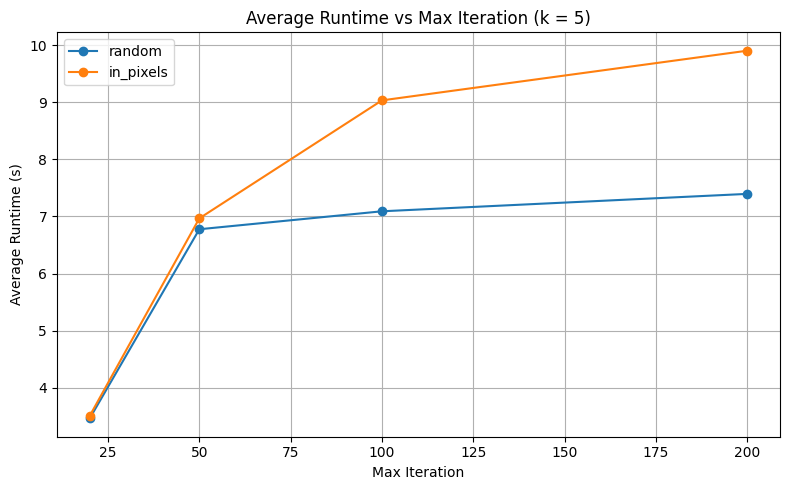
\includegraphics[width=0.48\linewidth]{imgs/benchmark/k5.png}
  }

  \subfloat[\(k = 7\)]{%
    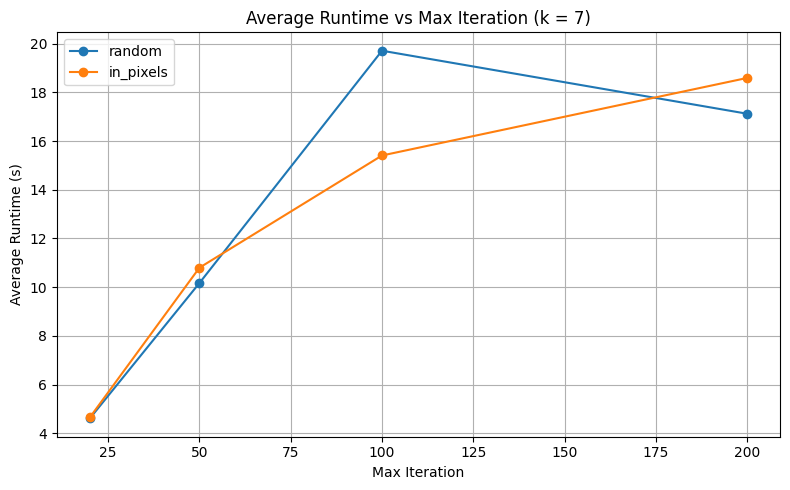
\includegraphics[width=0.48\linewidth]{imgs/benchmark/k7.png}
  }
  \hfill
  \subfloat[\(k = 9\)]{%
    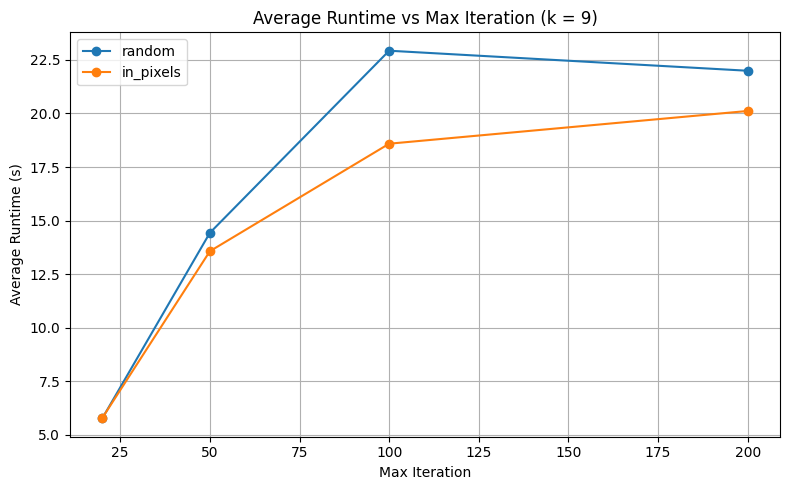
\includegraphics[width=0.48\linewidth]{imgs/benchmark/k9.png}
  }
  \caption{Thời gian thực thi trung bình với các giá trị số cụm \(k\) khác nhau}
  \label{fig:runtime_k}
\end{figure}


\subsection{Số vòng lặp hội tụ}

Qua quá trình benchmark với các giá trị \texttt{max\_iter} khác nhau (20, 50, 100, 200) và số cụm \(k\) đa dạng, có thể rút ra các nhận xét sau về số vòng lặp hội tụ của thuật toán k-means:

\begin{itemize}
  \item Với \texttt{max\_iter} thấp (20): hầu hết trường hợp không thể hội tụ trước khi đạt giới hạn. Điều này cho thấy 20 vòng thường quá ít để thuật toán ổn định với dữ liệu ảnh và các cấu hình \(k\) thông thường.
  \item Khi tăng \texttt{max\_iter} lên khoảng 50: tỉ lệ hội tụ trước ngưỡng tăng lên so với 20, nhưng vẫn còn nhiều trường hợp đặc biệt với \(k\) lớn hoặc khởi tạo không thuận lợi không kịp hội tụ. Các lần hội tụ (nếu có) thường ở khoảng 20–50 vòng.
  \item Với \texttt{max\_iter} ở mức 100: đa số trường hợp hội tụ trước ngưỡng, nhưng số vòng thực tế dao động rộng (có thể từ 20 đến gần 100), phụ thuộc vào \(k\) và cách khởi tạo centroid. Điều này cho thấy 100 vòng là mức hợp lý để hầu hết hội tụ, nhưng vẫn cần quan sát độ dao động của số vòng thực tế.
  \item Khi \texttt{max\_iter} đạt 200: phần lớn các trường hợp hội tụ, kể cả với \(k\) lớn, nhưng đôi khi số vòng cần thiết rất cao (gần 200). Do đó, mặc dù tăng ngưỡng giúp nâng khả năng hội tụ, chi phí tính toán cũng tăng đáng kể khi thuật toán cần nhiều vòng.
  \item Xu hướng chung: số vòng lặp hội tụ tăng theo \(k\). Với \(k\) nhỏ, thường hội tụ nhanh hơn; khi \(k\) lớn, cần nhiều vòng để centroid ổn định. Phương pháp khởi tạo cũng ảnh hưởng: khởi tạo từ pixel thực (\texttt{in\_pixels}) có thể giúp hội tụ nhanh hơn ở một số cấu hình, nhưng không hoàn toàn ổn định cho mọi \(k\).
  \item Khuyến nghị: để đảm bảo hội tụ, cần chọn \texttt{max\_iter} đủ cao (ít nhất 100) với ảnh trung bình; đồng thời nên cân nhắc khởi tạo thông minh (ví dụ k-means++) để giảm số vòng lặp thực tế.
\end{itemize}


\subsection{So sánh hai phương pháp khởi tạo centroid}

Dưới đây là phân tích dựa trên kết quả benchmark (thời gian trung bình) cho các kết hợp \texttt{max\_iter} = \{20, 50, 100, 200\} và số cụm \(k\) = \{3, 5, 7, 9\}. Bảng dữ liệu trung bình về thời gian thực thi (giây) như sau:

\begin{table}[H]
  \centering
  \caption{Thời gian thực thi trung bình (\texttt{avg\_time}) theo phương pháp khởi tạo centroid, cho từng \texttt{max\_iter} và \(k\).}
  \begin{tabular}{|c|c|c|c|c|c|}
    \toprule
    \texttt{max\_iter} & \(k\) & \texttt{random} & \texttt{in\_pixels} & Phương pháp nhanh hơn & Ghi chú                      \\
    \midrule
    20                 & 3     & 2.149           & 2.309               & random                & random nhanh hơn rõ          \\
    20                 & 5     & 3.465           & 3.509               & random                & chênh lệch nhỏ               \\
    20                 & 7     & 4.620           & 4.661               & random                & chênh lệch rất nhỏ           \\
    20                 & 9     & 5.773           & 5.792               & random                & chênh lệch rất nhỏ           \\
    \midrule
    50                 & 3     & 4.189           & 3.109               & in\_pixels            & in\_pixels nhanh hơn đáng kể \\
    50                 & 5     & 6.776           & 6.967               & random                & random nhanh hơn nhẹ         \\
    50                 & 7     & 10.172          & 10.801              & random                & random nhanh hơn             \\
    50                 & 9     & 14.431          & 13.572              & in\_pixels            & in\_pixels nhanh hơn         \\
    \midrule
    100                & 3     & 3.425           & 3.485               & random                & chênh lệch rất nhỏ           \\
    100                & 5     & 7.090           & 9.032               & random                & random nhanh hơn rõ          \\
    100                & 7     & 19.706          & 15.407              & in\_pixels            & in\_pixels nhanh hơn đáng kể \\
    100                & 9     & 22.930          & 18.590              & in\_pixels            & in\_pixels nhanh hơn rõ      \\
    \midrule
    200                & 3     & 3.650           & 3.416               & in\_pixels            & in\_pixels nhanh hơn nhẹ     \\
    200                & 5     & 7.395           & 9.902               & random                & random nhanh hơn đáng kể     \\
    200                & 7     & 17.120          & 18.589              & random                & random nhanh hơn nhẹ         \\
    200                & 9     & 21.995          & 20.118              & in\_pixels            & in\_pixels nhanh hơn         \\
    \bottomrule
  \end{tabular}
  \label{tab:compare_init}
\end{table}

Từ bảng trên, rút ra một số nhận xét chính:

\begin{itemize}
  \item \textbf{Với \texttt{max\_iter} = 20 (giới hạn thấp)}:
        \begin{itemize}
          \item Ở mọi \(k \in \{3,5,7,9\}\), \texttt{random} đều nhanh hơn \texttt{in\_pixels}, dù chênh lệch có khi rất nhỏ.
        \end{itemize}

  \item \textbf{Với \texttt{max\_iter} = 50 (vừa phải)}:
        \begin{itemize}
          \item Ở \(k=3\) và \(k=9\), \texttt{in\_pixels} nhanh hơn do khởi tạo ban đầu gần giá trị pixel thực, giúp hội tụ sớm.
          \item Ở \(k=5\) và \(k=7\), \texttt{random} vẫn nhỉnh hơn một chút, cho thấy khi \(k\) trung bình, khởi tạo ngẫu nhiên đôi khi phân bố centroid hợp lý hơn.
        \end{itemize}

  \item \textbf{Với \texttt{max\_iter} = 100 (cao hơn)}:
        \begin{itemize}
          \item Ở \(k=3\), hai phương pháp gần tương đương.
          \item Ở \(k=5\), \texttt{random} nhanh hơn rõ.
          \item Ở \(k=7\) và \(k=9\), \texttt{in\_pixels} nhanh hơn đáng kể, do khả năng khởi tạo gần vùng màu thực giúp giảm số vòng lặp khi \(k\) lớn.
        \end{itemize}

  \item \textbf{Với \texttt{max\_iter} = 200 (rất cao)}:
        \begin{itemize}
          \item Ở \(k=3\), \texttt{in\_pixels} nhanh hơn nhẹ.
          \item Ở \(k=5\) và \(k=7\), \texttt{random} nhanh hơn, cho thấy khởi tạo ngẫu nhiên giúp thuật toán tránh bị kẹt khi có nhiều màu trung bình/phức tạp.
          \item Ở \(k=9\), \texttt{in\_pixels} nhanh hơn, do khởi tạo từ dữ liệu thực giúp hội tụ nhanh trong không gian màu rất đa dạng.
        \end{itemize}

\end{itemize}

\paragraph{Kết luận tổng quát}
\begin{itemize}
  \item Không có phương pháp khởi tạo nào \emph{luôn} vượt trội trong mọi cấu hình.
  \item \texttt{in\_pixels} có xu hướng \emph{ổn định và nhanh hơn} khi \(k\) rất nhỏ (3) hoặc rất lớn (9) ở một số ngưỡng vòng lặp đủ cao (50, 100, 200).
  \item \texttt{random} thường chiếm ưu thế ở \(k\) trung bình (5, 7) trong nhiều trường hợp, nhất là khi \texttt{max\_iter} không quá thấp, nhờ khả năng phân bố centroid ban đầu rộng hơn, tránh khởi tạo trùng vùng màu nhiều.
  \item Khi \texttt{max\_iter} quá thấp (20), \texttt{random} thường nhanh hơn vì thuật toán có ít vòng để điều chỉnh, và khởi tạo ngẫu nhiên đôi khi may mắn phân bố tốt hơn.
  \item Tính ổn định: \texttt{in\_pixels} ít dao động hơn với các \(k\) rất nhỏ hoặc rất lớn, nhưng với \(k\) trung bình có thể bị khởi tạo trùng vùng màu, làm chậm. \texttt{random} dao động mạnh hơn nhưng không dễ bị kẹt lâu ở \(k\) trung bình.
\end{itemize}

\paragraph{Gợi ý thực tiễn}
\begin{itemize}
  \item Với ảnh có phân bố màu \emph{đơn giản, ít màu} hoặc khi cần số cụm rất nhỏ (\(k=3\)), ưu tiên \texttt{in\_pixels} để hội tụ nhanh.
  \item Với ảnh có \emph{màu trung bình/phức tạp} (số lượng màu và sắc độ tương đối đa dạng) và \(k\) trung bình (5–7), \texttt{random} thường hiệu quả hơn.
  \item Với \(k\) rất lớn (\(\geq9\)) và giới hạn vòng lặp đủ cao, \texttt{in\_pixels} có thể cho thời gian thực thi tốt hơn, nhưng cần lưu ý kiểm tra tính ổn định (nên chạy nhiều lần với seed khác nhau).
  \item Luôn cân nhắc sử dụng khởi tạo \texttt{k-means++} trong thực tế để giảm rủi ro khởi tạo kém và cải thiện hội tụ chung cho mọi \(k\).
\end{itemize}


\subsection{Giới hạn và vấn đề gặp phải}

Trong quá trình thực nghiệm và benchmark, một số giới hạn và vấn đề sau được ghi nhận:

\begin{itemize}
  \item \textbf{Quy mô và đa dạng của tập ảnh}: Bộ benchmark sử dụng số lượng hạn chế (khoảng 10 ảnh) với độ phân giải đã resize về mức cố định. Chưa đánh giá được hiệu năng với tập ảnh lớn, độ phân giải rất cao hoặc đa dạng hoàn cảnh nhiễu, ánh sáng, làm giảm tính khái quát của kết quả.
  \item \textbf{Khả năng hội tụ không đảm bảo ở ngưỡng thấp}: Với \texttt{max\_iter} thấp (ví dụ 20), đa phần trường hợp không hội tụ kịp, cho thấy ngưỡng vòng lặp cần đủ cao (\(\geq50\)–100) để đảm bảo thuật toán ổn định với nhiều cấu hình \(k\).
  \item \textbf{Độ nhạy với khởi tạo centroid}: Cả hai phương pháp (\texttt{random}, \texttt{in\_pixels}) đôi khi gặp trường hợp khởi tạo không thuận lợi, dẫn tới số vòng lặp lớn hoặc không hội tụ trong giới hạn. Điều này cho thấy cần khởi tạo thông minh hơn (ví dụ k-means++).
  \item \textbf{Chi phí tính toán khi \(k\) và \texttt{max\_iter} cao}: Khi số cụm \(k\) tăng (\(\geq 7\)) và \texttt{max\_iter} lên đến 100–200, thời gian thực thi tăng rất nhanh, đôi khi tới vài chục giây cho mỗi ảnh. Điều này đặt áp lực về tài nguyên và thời gian, nhất là khi xử lý nhiều ảnh hoặc độ phân giải cao.
\end{itemize}

\subsection{Kết luận}

Qua quá trình thực nghiệm và phân tích kết quả, có thể rút ra một số kết luận chính về thuật toán K-Means trong nén màu ảnh:

\begin{itemize}
  \item \textbf{Ảnh hưởng của tham số \(k\) và max\_iter}: Thời gian thực thi và số vòng lặp hội tụ tăng rõ khi số cụm \(k\) lớn (\(\geq7\)) và khi ngưỡng \texttt{max\_iter} đủ cao (\(\geq100\)). Ngưỡng quá thấp (20) thường không đảm bảo hội tụ, ngưỡng ở mức vừa phải (50) cải thiện nhưng chưa chắc đã hội tụ với mọi cấu hình, và mức \(\geq100\)–200 là cần thiết để đa số trường hợp hội tụ.
  \item \textbf{So sánh khởi tạo centroid}:
        \begin{itemize}
          \item Phương pháp \texttt{in\_pixels} tỏ ra hội tụ nhanh hơn và ổn định hơn trong nhiều trường hợp với \(k\) rất nhỏ (3) hoặc rất lớn (9) khi ngưỡng vòng lặp đủ cao, nhờ khởi tạo gần giá trị pixel thực.
          \item Phương pháp \texttt{random} linh hoạt hơn với \(k\) trung bình (5–7) và có thể tránh việc chọn centroid ban đầu trùng vùng màu nhiều, nhưng đôi khi cần nhiều vòng lặp hơn hoặc không hội tụ kịp ở ngưỡng thấp.
          \item Cả hai cách đều có nhược điểm khi khởi tạo kém, do đó không có phương pháp nào luôn tối ưu tuyệt đối cho mọi loại ảnh.
        \end{itemize}
  \item \textbf{Ưu tiên khởi tạo thông minh}: Kết quả nhấn mạnh tầm quan trọng của phương pháp khởi tạo như \emph{k-means++}, giúp phân bố centroid ban đầu hiệu quả hơn, giảm số vòng lặp và tăng xác suất hội tụ.
  \item \textbf{Cân bằng hiệu năng và chất lượng}: Trong thực tế, cần cân nhắc chọn \(k\) hợp lý (thường 5–9 cho nhiều bài toán nén màu) và đặt \texttt{max\_iter} đủ cao (\(\geq 100\)) để đảm bảo hội tụ, đồng thời kiểm soát chi phí tính toán (có thể giảm độ phân giải hoặc trích mẫu điểm).
  \item \textbf{Tối ưu triển khai}: Để áp dụng trên tập lớn hoặc ảnh độ phân giải cao, nên kết hợp song song hóa, vectorization.
\end{itemize}





